% !TeX spellcheck = nl_NL
\documentclass[a4paper,kul]{kulakarticle} %options: kul or kulak (default)

\usepackage[utf8]{inputenc}
\usepackage[dutch]{babel}

\date{Academiejaar 2021 -- 2022}
\address{
	Industriële Ingenieurswetenschappen \\
	BioTechnologie \\
	Inge Holsbeeks \& Hans Rediers}
\title{Samenvatting}
\author{Robbe Decapmaker}
\usepackage{hyperref}
\usepackage{graphicx}
\usepackage{amsmath, amssymb, amsthm}
\usepackage{siunitx}
\usepackage{flafter} 
\usepackage{pdfpages}
\usepackage{caption}
\usepackage{subcaption}
\usepackage{titlesec}

\setcounter{secnumdepth}{4}

\titleformat{\paragraph}
{\normalfont\normalsize\bfseries}{\theparagraph}{1em}{}
\titlespacing*{\paragraph}
{0pt}{3.25ex plus 1ex minus .2ex}{1.5ex plus .2ex}


\begin{document}

\maketitle

\section*{Inleiding}

De samenvatting van BioTechnologie. \href{https://github.com/debber1/BioTech}{De source code is te vinden op Github.}\\
%DEZE ZIN IS ENKEL RELEVANT TIJDENS DE ONTWIKKELING VAN DIT DOCUMENT
\textbf{Dit document is een `work in progress', dit wil zeggen dat er (ongeveer) een wekelijkse update zal zijn. De meest recente versie zal altijd op Github staan!}
\tableofcontents
\newpage
\section{Koolhydraten}
Koolhydraten zijn essentieel voor biologisch leven. Grosso modo kunnen we 3 verschillende types onderscheiden: monosachariden, disachariden en polysachariden. Voor dat we deze types degelijk kunnen bespreken moet er eerst enkele afspraken vast gelegd worden rond naamgeving een voorstelling. We moeten ook nog enkele belangrijke opmerken maken rond de chemische fenomenen die zich voor doen bij koolhydraten. 
\subsection{Naamgeving}
Koolhydraten bestaan voornamelijk uit C, O en H atomen. Afhankelijk van de onderling gevormde bindingen kunnen we een onderscheid maken tussen twee soorten koolhydraten; de aldosen en ketonen. Het verschil tussen beiden wordt duidelijk gemaakt in figuur \ref{fig:aldehyde-keton}. Als een koolhydraat in bezit is van een aldehyde groep, noemen we hem een aldose. Als hij in bezit is van een keton groep, noemen we hem een ketose.
\begin{figure}[htbp]
	\centering
	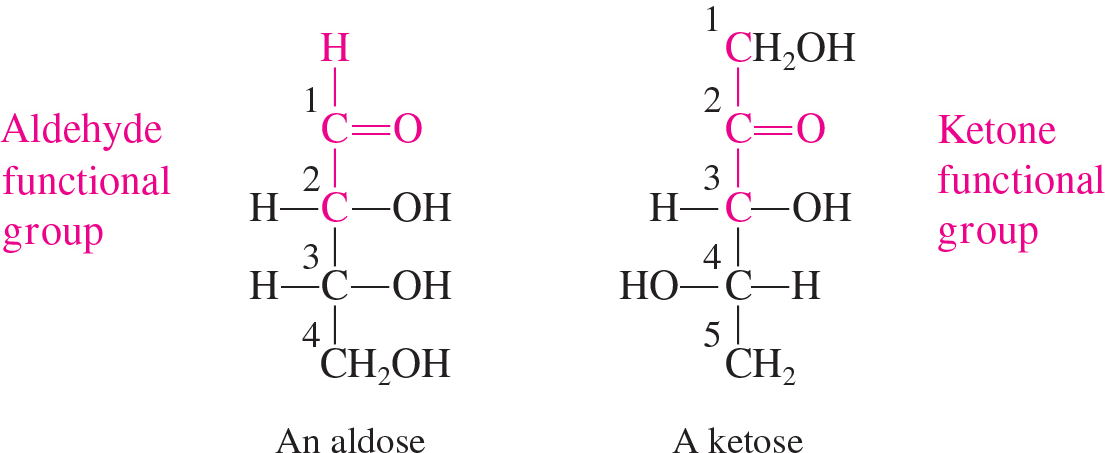
\includegraphics[width=0.7\linewidth]{Aldehyde-Keton}
	\caption[Aldehyden en ketonen]{Aldehyden en ketonen}
	\label{fig:aldehyde-keton}
\end{figure}\\
Naast de aanwezigheid van functionele groepen, maken we ook een onderscheid op basis van het aantal aanwezige koolstof atomen. De nummering en naamgeving van deze moleculen worden overgenomen uit de chemie zoals te zien is op figuur \ref{fig:examples-name}.
\begin{figure}[htbp]
	\centering
	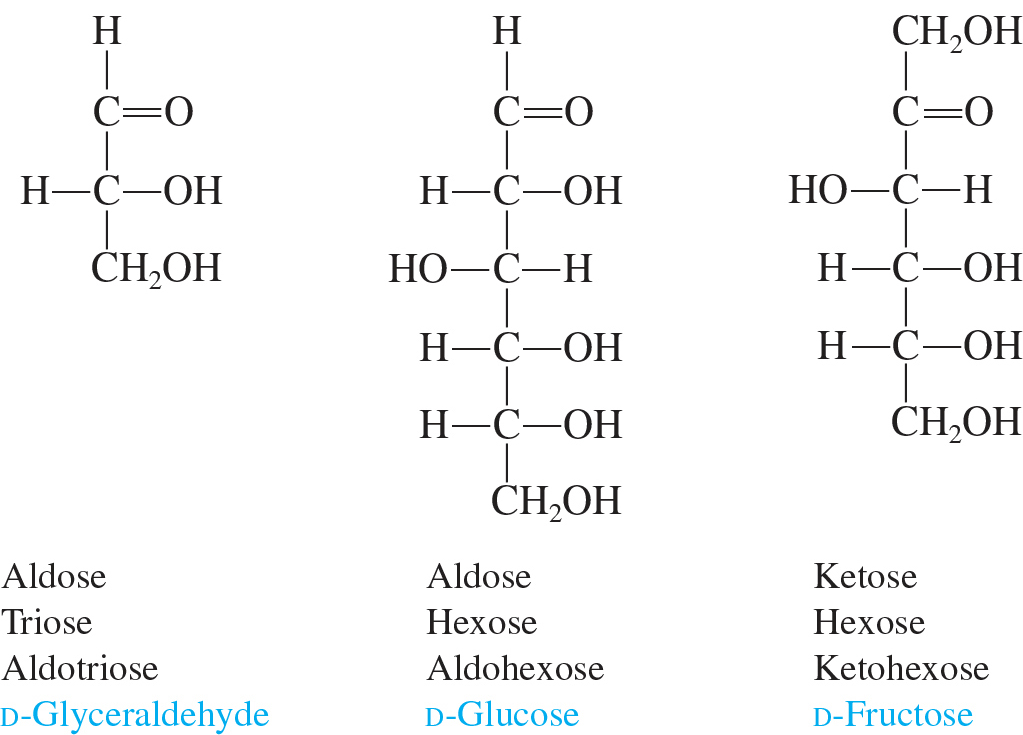
\includegraphics[width=0.6\linewidth]{examples-name}
	\caption[Naamgeving]{Voorbeelden van naamgeving}
	\label{fig:examples-name}
\end{figure}\\
Er zijn ook enkele koolhydraten die een triviale naam krijgen, zoals sacharose of fructose.

\subsection{Voorstellingen}
Er bestaan twee manieren om een koolhydraat voor te stellen, de Fischer- en Haworthprojectie. Voor D-glucose zien we op figuur \ref{fig:fishervshaworth} beide voorstellingen.
\begin{figure}[h]
	\centering
	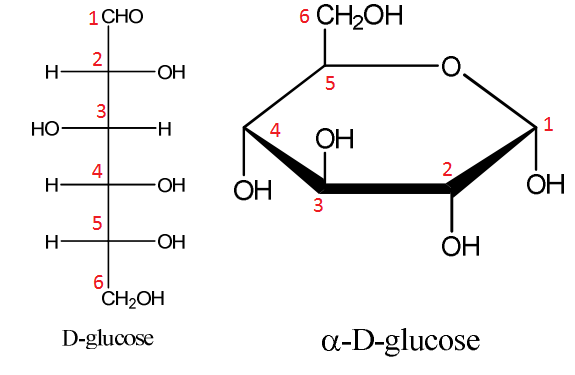
\includegraphics[width=0.6\linewidth]{FisherVSHaworth}
	\caption[Fischer- en Haworthprojectie]{Fischerprojectie (links) en Haworthprojectie (rechts)}
	\label{fig:fishervshaworth}
\end{figure}

\subsection{Stereochemie}
Als de structuur van een koolhydraat koolstof atomen bevat die gebonden zijn met vier verschillende groepen, zeggen we dat de structuur een chiraal centrum heeft. Dit fenomeen kan tot opmerkelijke resultaten leiden, zo is het mogelijk da bepaalde functionele groepen niet altijd op dezelfde manier georiënteerd zijn.  
\subsubsection{Enantiomeren}
We spreken van enantiomeren als een we te maken hebben met een molecule die volledig gespiegeld kan worden. Een voorbeeld is te zien op figuur \ref{fig:enantiomeren}. Deze spiegeling heeft enkele gevolgen, zowel op biologisch als op fysisch vlak. Zo kunnen verschillende enantiomeren anders reageren op gepolariseerd licht. Vanuit een biologisch standpunt vormt er een probleem als de enantiomeren niet op dezelfde manier samenwerken met enzymen (zie figuur \ref{fig:enantiomeerenzym}). Als beide enantiomeren (normaal en gespiegeld of L en D in een biologische context) aanwezig zijn in een mengsel, dan nomen we dit een racemisch mengsel.
Het is ook belangrijk om op te merken dat een gespiegelde tekening niet zomaar een enantiomeer is. Het is ook mogelijk dat er een mesoverbinding aan het werk is. Dit is een verbinding met twee of meer chirale koolstofatomen en een intern symmetrievlak zoals te zien is op figuur \ref{fig:mesoverbinding}. 
\begin{figure}
	\centering
	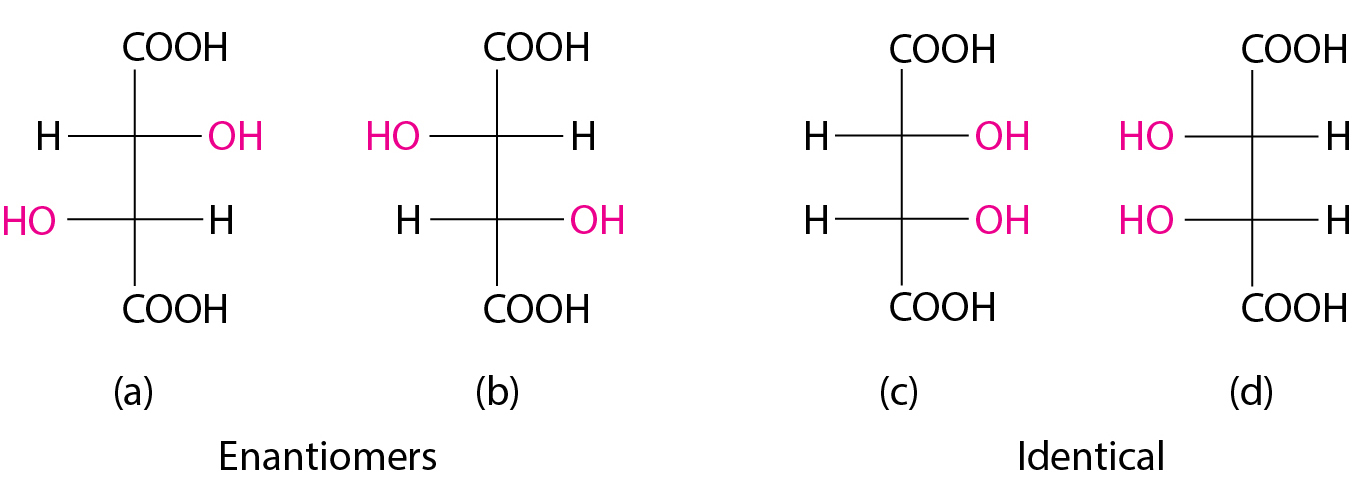
\includegraphics[width=0.7\linewidth]{mesoverbinding}
	\caption[Mesoverbinding]{Enantiomeer (links) en mesoverbinding (rechts)}
	\label{fig:mesoverbinding}
\end{figure}

\begin{figure}[htbp]
	\centering
	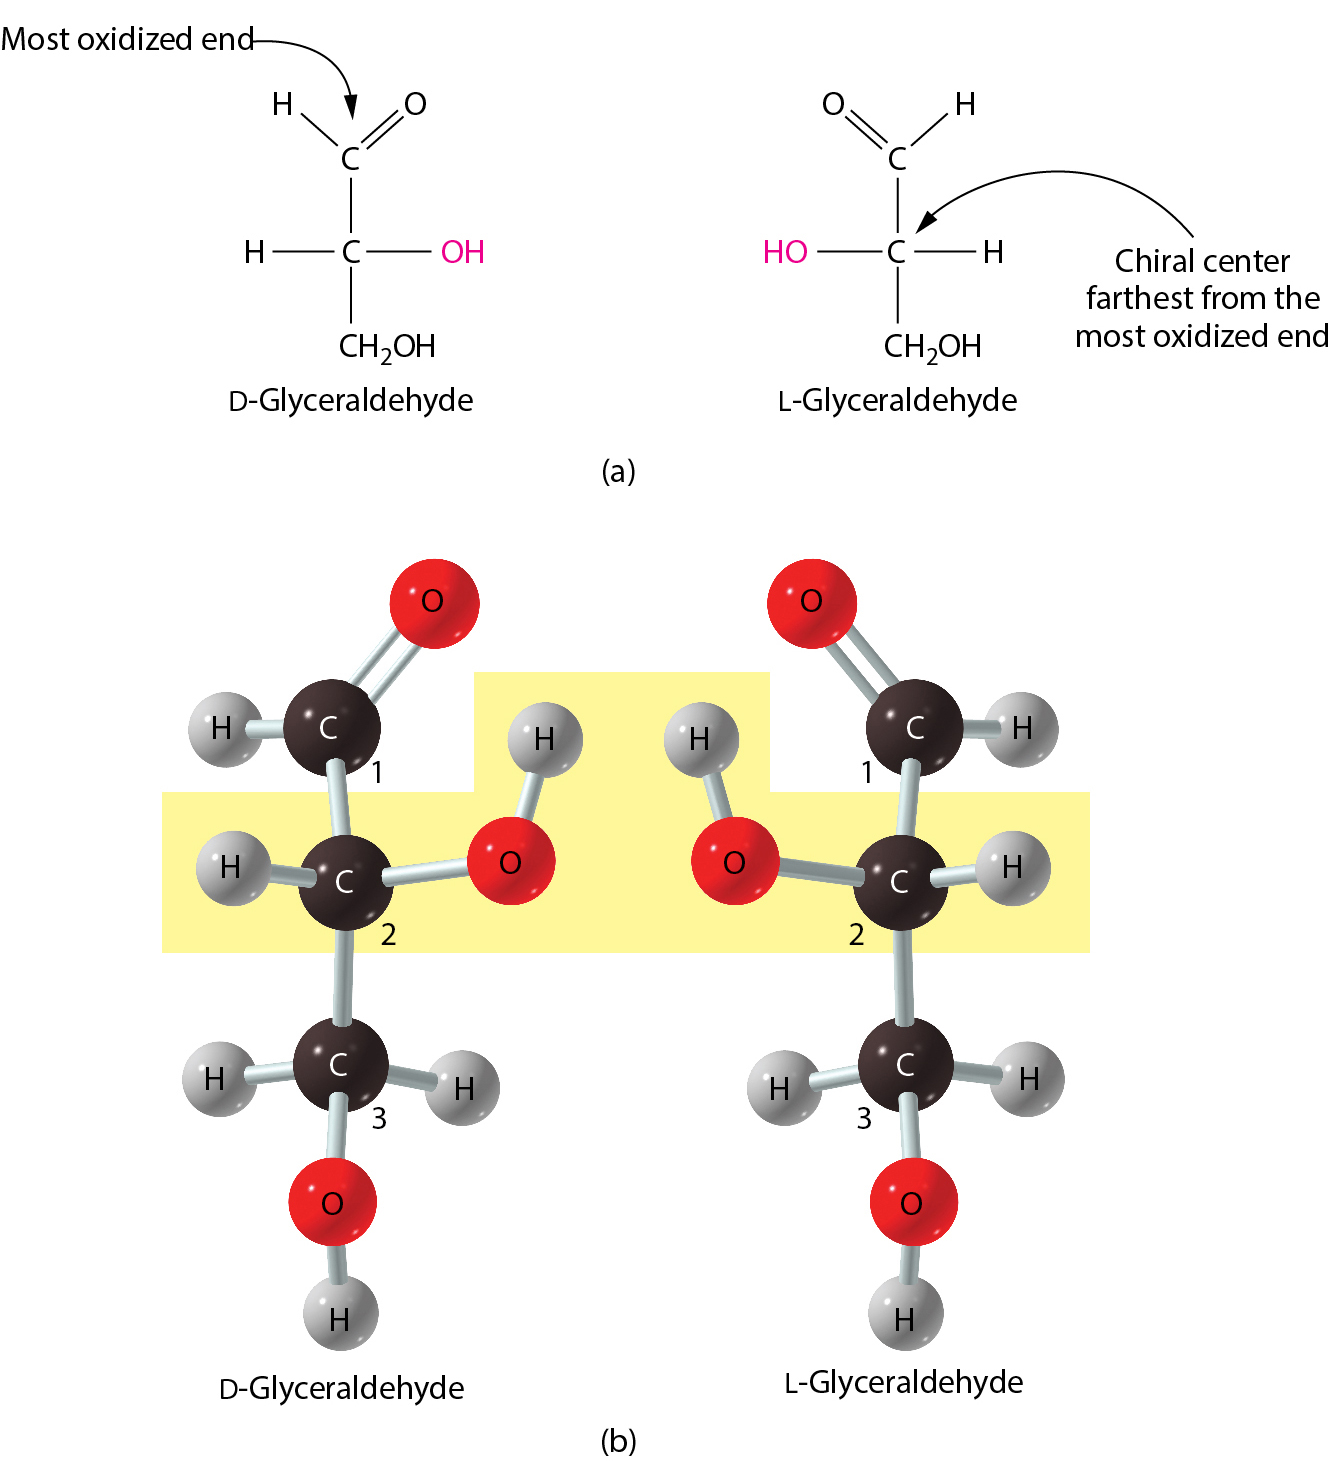
\includegraphics[width=0.6\linewidth]{enantiomeren}
	\caption[Enantiomeer]{Enantiomeer}
	\label{fig:enantiomeren}
\end{figure}
\begin{figure}[htbp]
	\centering
	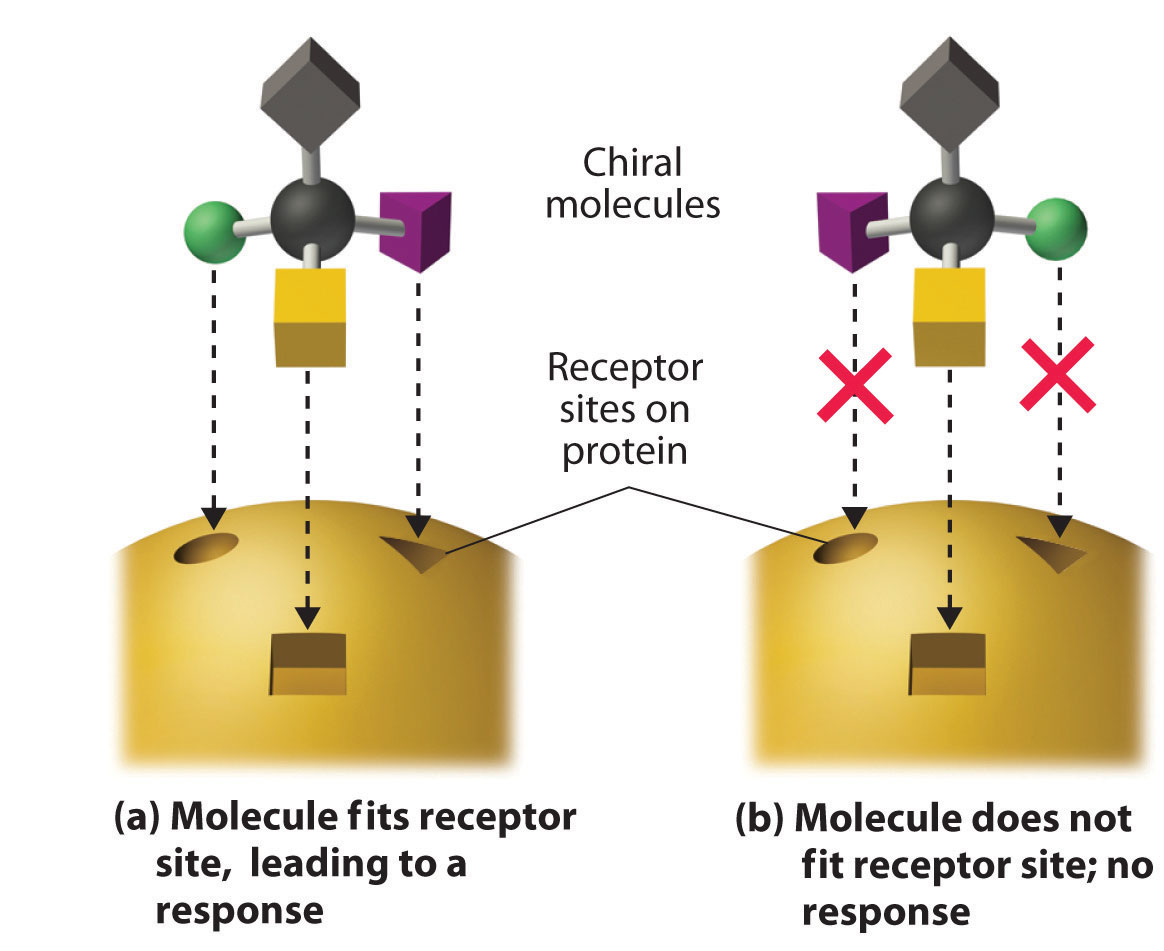
\includegraphics[width=0.5\linewidth]{EnantiomeerEnzym}
	\caption[Enantiomeer en enzym]{Interactie tussen enantiomeren en enzymen}
	\label{fig:enantiomeerenzym}
\end{figure}


\subsubsection{Diastereomeren}
\begin{figure}[htbp]
	\centering
	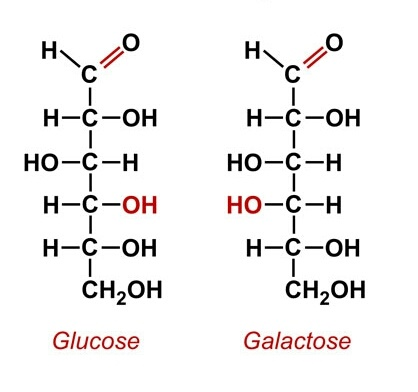
\includegraphics[width=0.4\linewidth]{Diastereomeren}
	\caption[Diastereomeren]{Diastereomeren}
	\label{fig:diastereomeren}
\end{figure}
Diastereomeren zijn zoals enantiomeren, maar ze zijn geen perfect spiegelbeeld zoals te zien is op figuur \ref{fig:diastereomeren}.
\subsubsection{Glucose}
Het bekendste voorbeeld van deze fenomenen is glucose. In de natuur observeren we D-glucose en L-glucose. Hiervan zien we hoofdzakelijk D-glucose voorkomen omdat dit het type glucose is dat gemaakt wordt door fotosynthese. Ons lichaam maakt wel een onderscheid tussen beide varianten, ze smaken alle twee zoet maar enkel D-glucose heeft een calorische inhoud bij het verteren. Dit wil zeggen dat L-glucose niet wordt opgenomen door ons spijsverterings-stelsel, en dus niet kan  gebruikt worden om energie uit te halen. Het is dus een `zoetstof'.

\subsection{Reducerende koolhydraten}
We spreken van een reducerend koolhydraat als het molecuul optreedt als reducerend agens in een reactie als gevolg van de aanwezigheid van de aldehyde- of ketongroep (zie figuur \ref{fig:reductiefding}). Veel monosachariden bezitten deze eigenschap, daarnaast hebben ook disachariden, waarvan het anomere koolstof-atoom geen glycoside binding heeft, ook een reducerend vermogen. Polysachariden hebben meestal een te lage hoeveelheid reducerende uiteinden om een reductief karakter te hebben.
\begin{figure}[htbp]
	\centering
	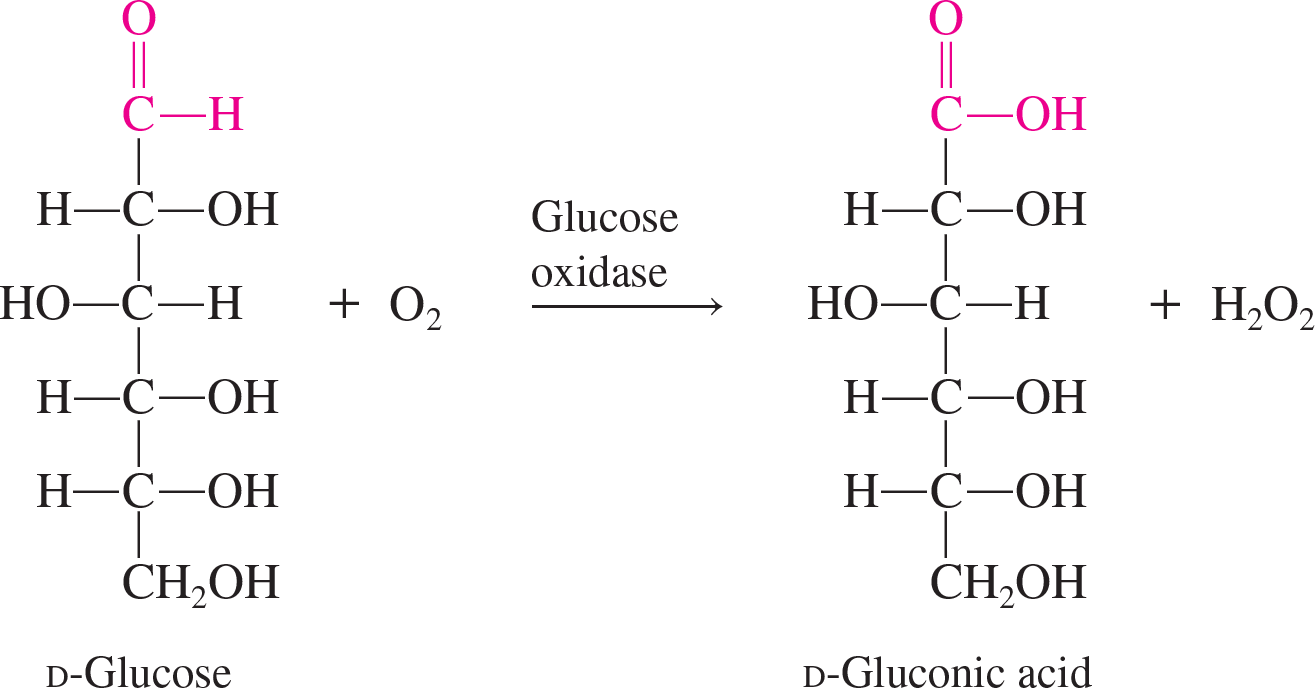
\includegraphics[width=0.5\linewidth]{ReductiefDing}
	\caption[Reducerende koolhydraten]{Reducerende koolhydraten}
	\label{fig:reductiefding}
\end{figure}\\
We kunnen testen of een koolhydraat in het bezit is van een reducerend karakter met Benetict's reagens. Hierbij kijken we naar de kleurverandering van de oplossing na de reactie. Dit is tevens de manier waarop we kunnen bepalen of er suiker in urine zit, het is handig om suikerziekte op te sporen.

\subsection{Monosachariden}
Monosachariden zijn de meest eenvoudige koolhydraten. Ze vormen hierdoor dus ook de bouwstenen voor complexere structuren zoals disachariden en polysachariden. 
\subsubsection{Belangrijke monosachariden}
\textbf{Glucose}
\begin{figure}[h]
	\centering
	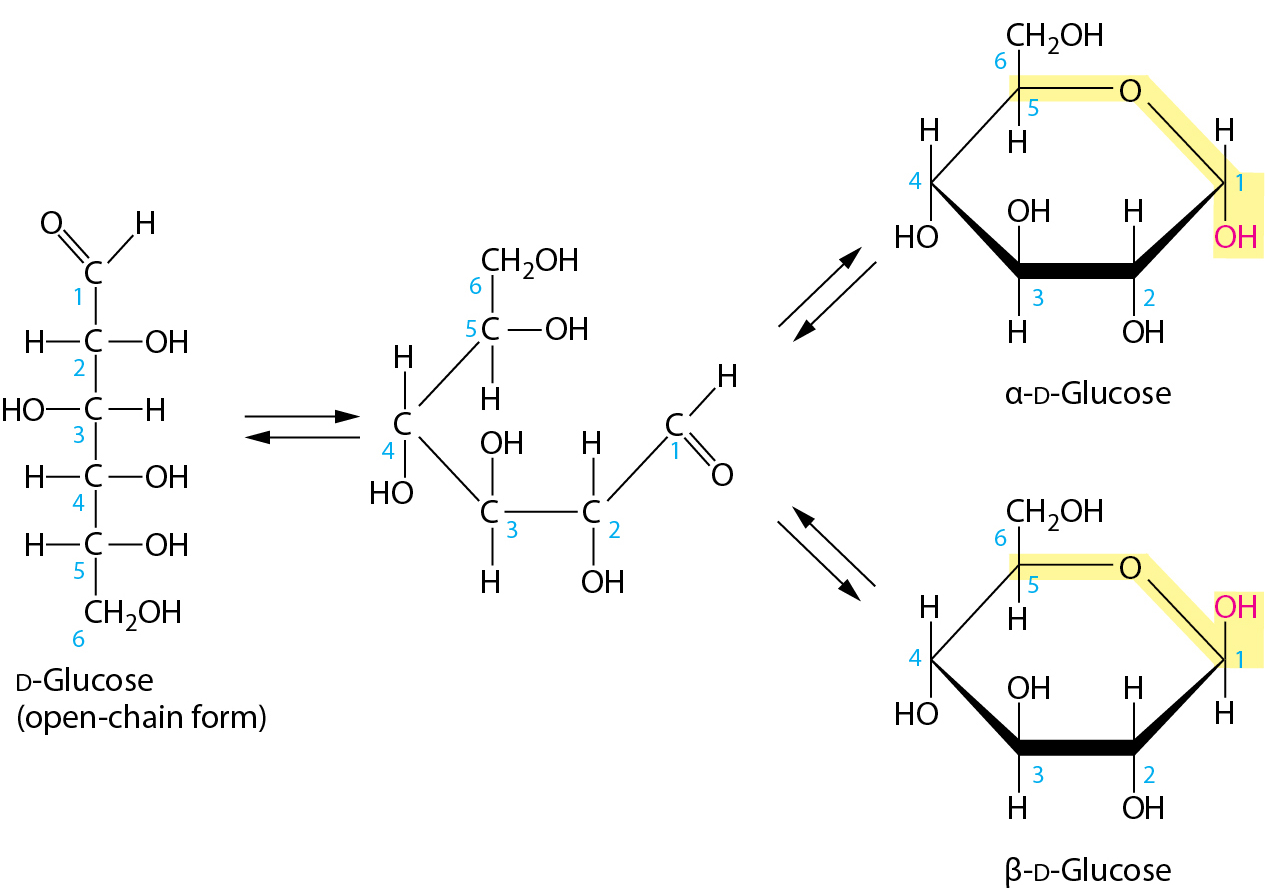
\includegraphics[width=0.7\linewidth]{GlucoseAlphaBeta}
	\caption[Glucose]{Glucose}
	\label{fig:glucosealphabeta}
\end{figure}\\
Hierbij kunnen we nog vermelden dat koolstof atoom 1 in figuur \ref{fig:glucosealphabeta} een nieuw chiraal centrum is, en dus een anomeer C-atoom is.\\
\textbf{Fructose}
\begin{figure}[h]
	\centering
	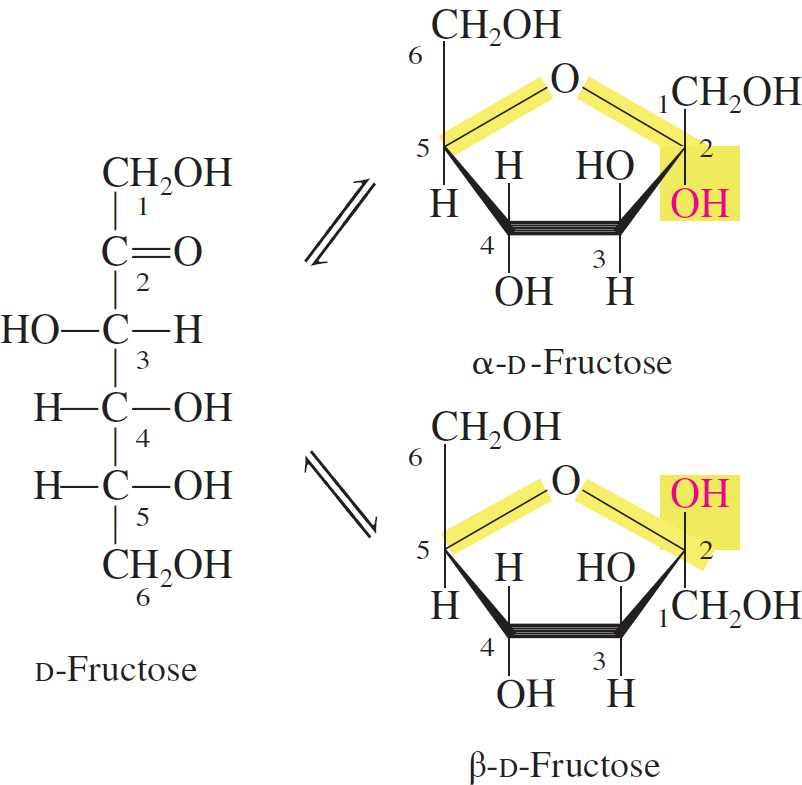
\includegraphics[width=0.4\linewidth]{FructoseAlphaBeta}
	\caption[Fructose]{Fructose}
	\label{fig:fructosealphabeta}
\end{figure}\\
Hierbij kunnen we nog vermelden dat koolstof atoom 2 in figuur \ref{fig:fructosealphabeta} een nieuw chiraal centrum is, en dus een anomeer C-atoom is.\\
\newpage
\textbf{Deoxyribose}
\begin{figure}[h]
	\centering
	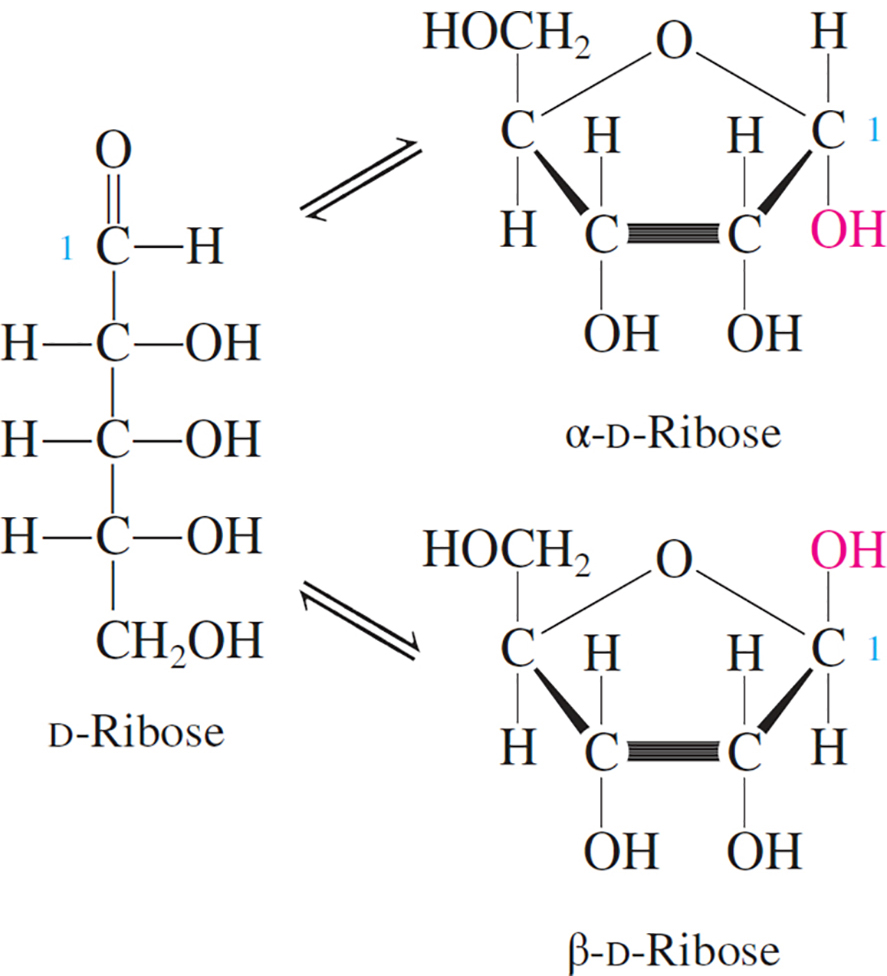
\includegraphics[width=0.4\linewidth]{deoxyribosealphabeta}
	\caption[Deoxyribose]{Deoxyribose}
	\label{fig:deoxyribosealphabeta}
\end{figure}\\
Hierbij kunnen we nog vermelden dat koolstof atoom 1 in figuur \ref{fig:deoxyribosealphabeta} een nieuw chiraal centrum is, en dus een anomeer C-atoom is. Deoxyribose is tevens belangrijk voor RNA en DNA.\\
\textbf{Acetylglucosamine}\\
Door andere functionele groepen toe te voegen aan de koolhydraatstructuur kunnen we complexere moleculen maken. Acetylglucosamine (figuur \ref{fig:acetylglucosamine}) is bijvoorbeeld een bloed antigen.
\begin{figure}[h]
	\centering
	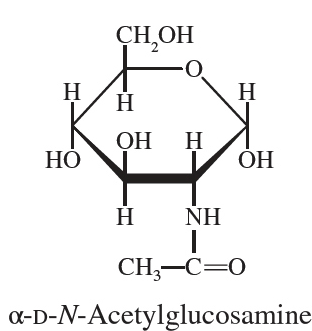
\includegraphics[width=0.4\linewidth]{Acetylglucosamine}
	\caption[Acetylglucosamine]{Acetylglucosamine}
	\label{fig:acetylglucosamine}
\end{figure}
\subsubsection{Afgeleiden}
Enkele voorbeelden van afgeleiden van monosachariden zijn polyolen. Ze zijn geen monosachariden, maar lijken er wel sterk op. De voorbeelden uit figuur \ref{fig:afgeleidenmonosachariden} zijn zoet zoals glucose, ze hebben wel geen calorie-inhoud. Ze zijn dus geschikt om zoetstoffen mee te maken.
\begin{figure}[h]
	\centering
	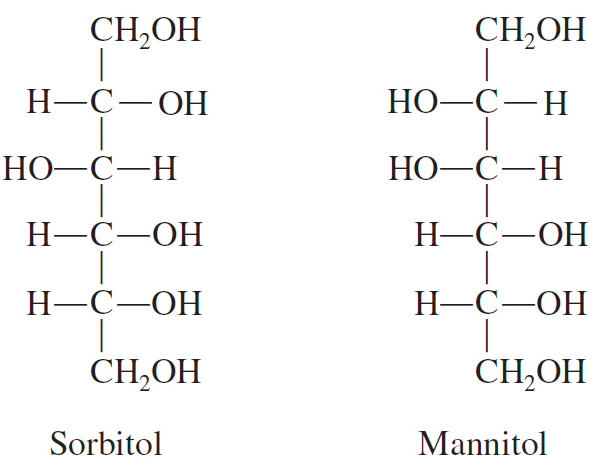
\includegraphics[width=0.4\linewidth]{AfgeleidenMonosachariden}
	\caption[Afgeleiden]{Afgeleiden van monosachariden}
	\label{fig:afgeleidenmonosachariden}
\end{figure}

\subsection{Disachariden}
Disachariden zijn opgebouwd uit 2 monosachariden. We kunnen ze benoemen volgens de monosachariden waaruit ze zijn opgebouwd, en de manier waarop deze gebonden zijn aan elkaar.
\subsubsection{Belangrijke disachariden}
\textbf{Sucrose}\\
Sucrose is wat wij kennen als 'gewoon' suiker. Het is opgebouwd uit $\alpha$-glucose en $\beta$-Fructose (zie figuur \ref{fig:sucrose}).
\begin{figure}[h]
	\centering
	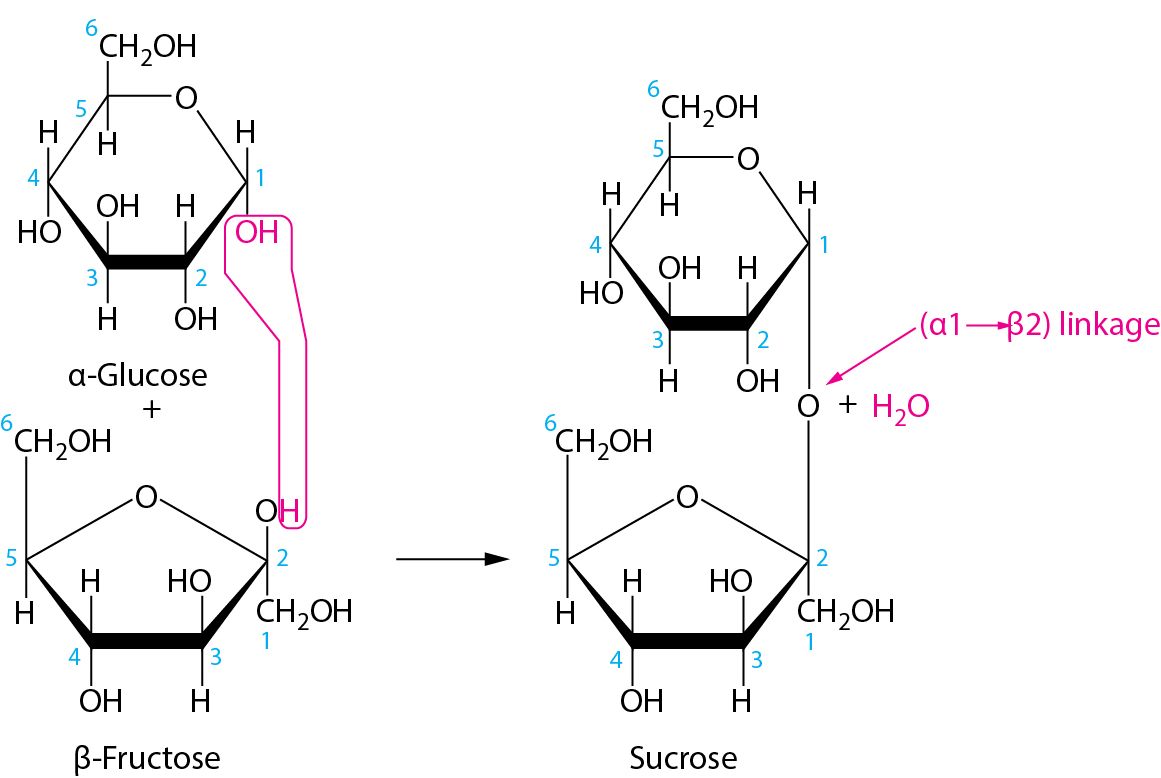
\includegraphics[width=0.5\linewidth]{sucrose}
	\caption[Sucrose]{Sucrose}
	\label{fig:sucrose}
\end{figure}\\
\textbf{Lactose}\\
Lactose of melksuiker is opgebouwd uit $\beta$-D-galactose en $\beta$-D-glucose (zie figuur \ref{fig:lactose}).
\begin{figure}[h]
	\centering
	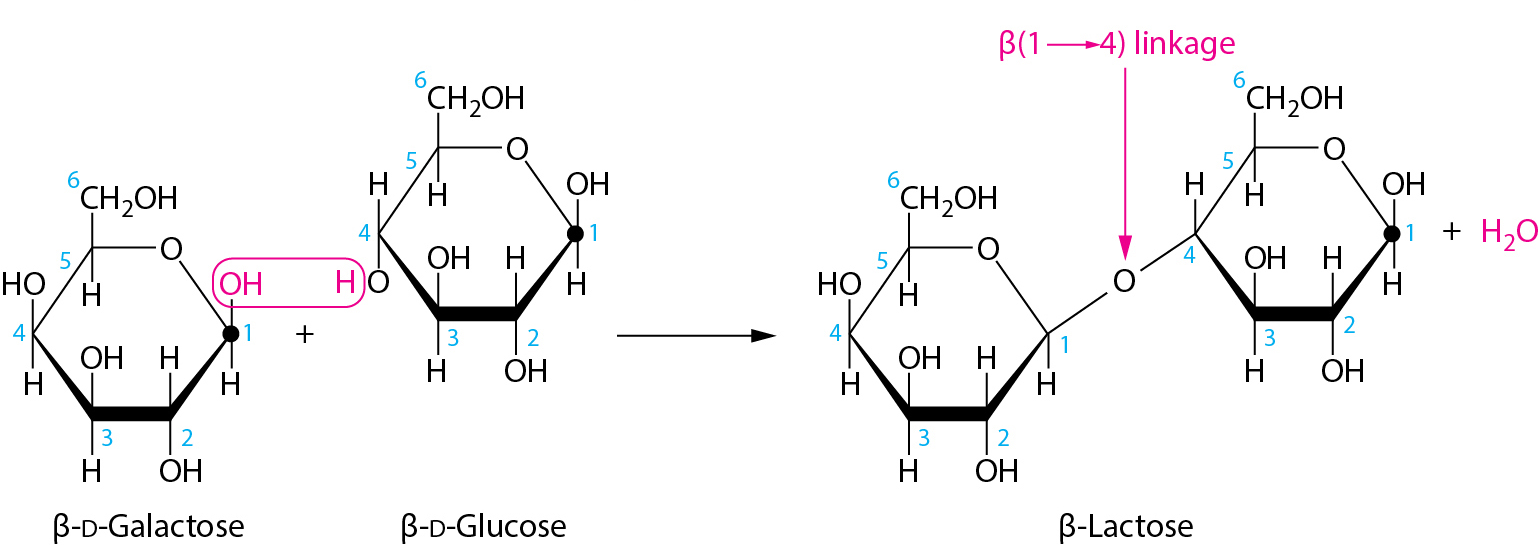
\includegraphics[width=0.6\linewidth]{Lactose}
	\caption[Lactose]{Lactose}
	\label{fig:lactose}
\end{figure}\\
\textbf{Maltose}\\
Maltose of moutsuiker is opgebouwd uit $\alpha$-D-glucose en $\beta$-D-glucose (zie figuur \ref{fig:maltose}).
\begin{figure}[h]
	\centering
	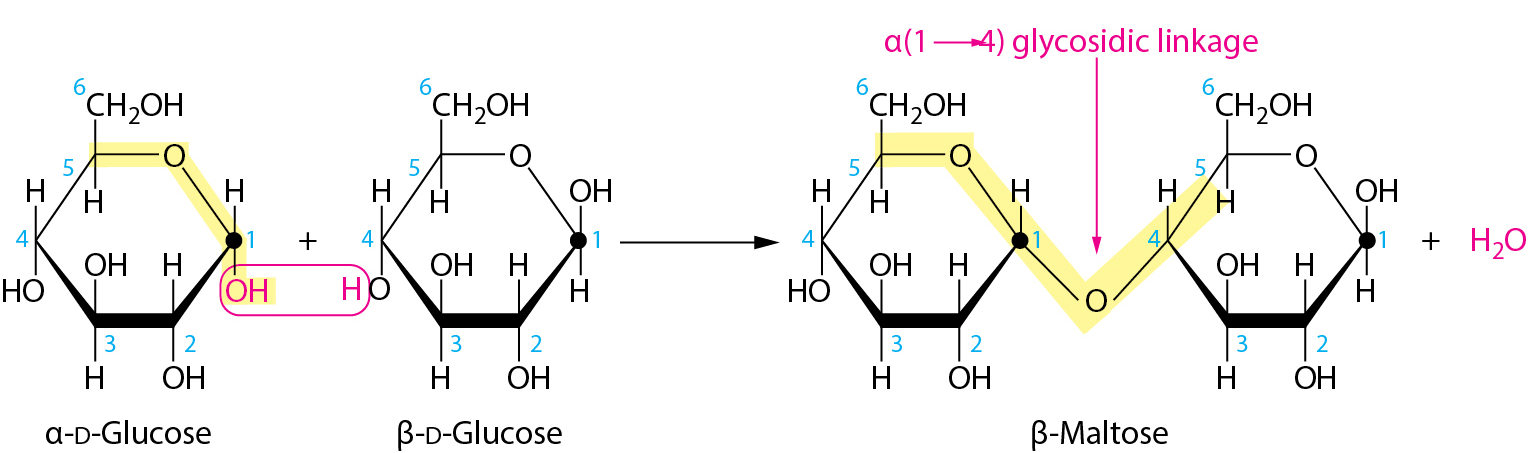
\includegraphics[width=0.6\linewidth]{Maltose}
	\caption[Maltose]{Maltose}
	\label{fig:maltose}
\end{figure}

\subsection{Polysachariden}
Polysachariden zijn net zoals disachariden opgebouwd uit monosachariden. Het verschil zit in de hoeveelheid bouwblokken er aanwezig zijn. Grosso modo zullen we spreken over polysachariden als er meer dan 2 monosachariden betrokken zijn bij de opbouw.

Afhankelijk van de onderlinge bindingen, kunnen er zich vertakkingen voor doen in een polysacharide. beide polysachariden in figuur \ref{fig:vertakkingen} zijn opgebouwd volgens de structuur in figuur \ref{fig:vertakking}. Door het aanzienlijke verschil in vertakkingen, maken we een onderscheid tussen deze twee moleculen.
\begin{figure}[h]
	\centering
	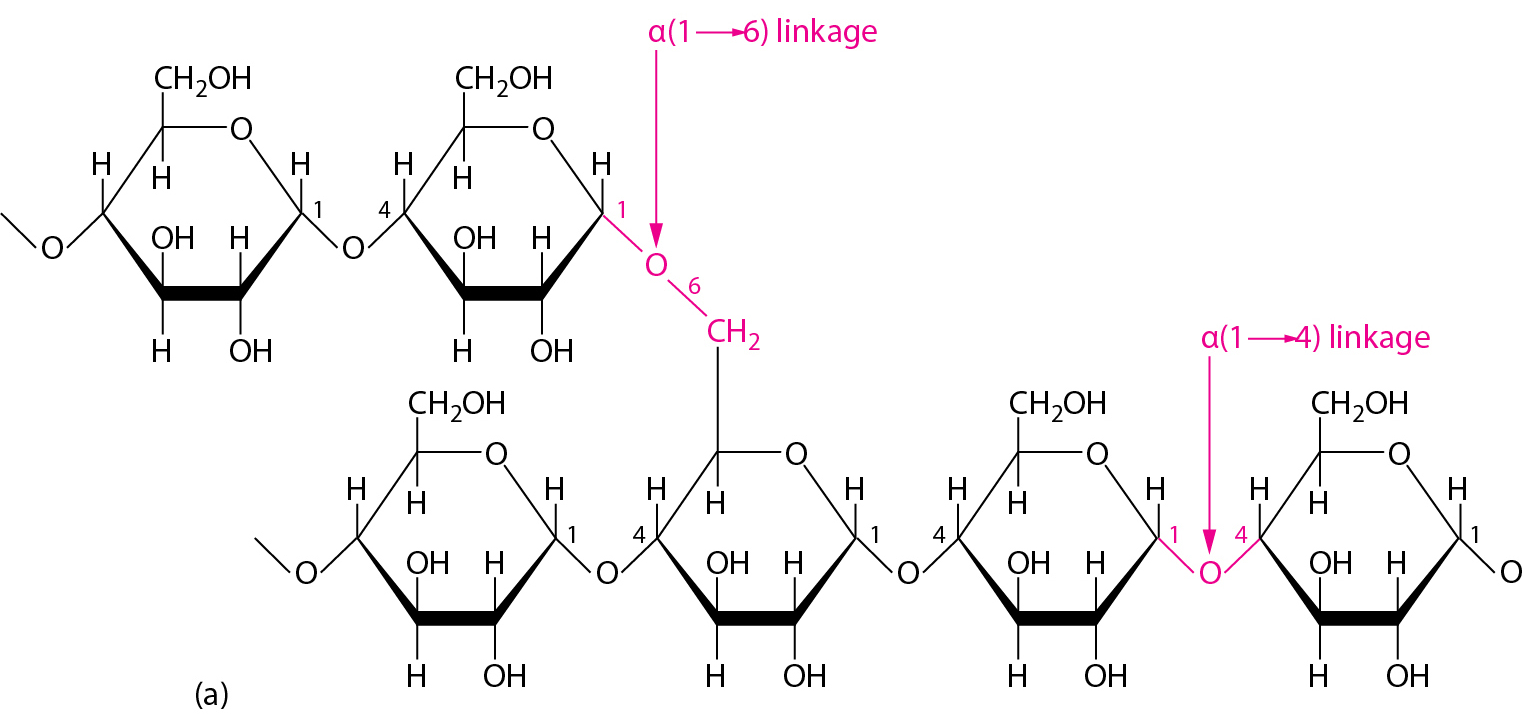
\includegraphics[width=0.7\linewidth]{Vertakking}
	\caption[Vertakking]{Verschillende bindingen zorgen voor vertakkingen}
	\label{fig:vertakking}
\end{figure}

\begin{figure}[h]
	\centering
	\begin{subfigure}{.5\textwidth}
		\centering
		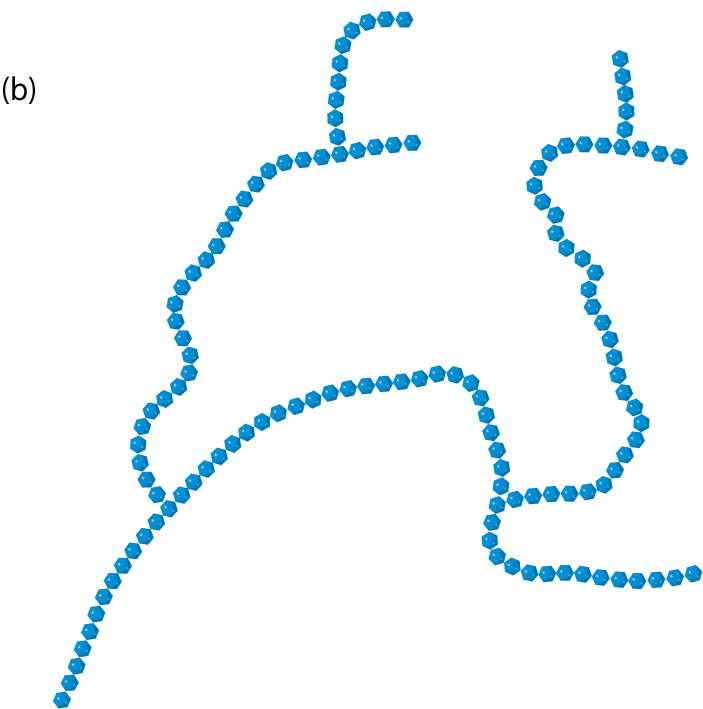
\includegraphics[width=.4\linewidth]{amylopectine_in_zetmeel.png}
		\caption{Amylopectine in zetmeel}
		\label{fig:sub1}
	\end{subfigure}%
	\begin{subfigure}{.5\textwidth}
		\centering
		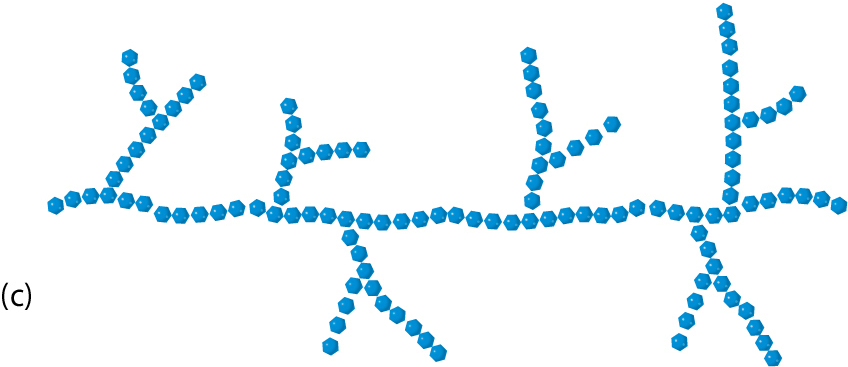
\includegraphics[width=.7\linewidth]{Glycogeen.png}
		\caption{Glycogeen}
		\label{fig:sub2}
	\end{subfigure}
	\caption{Het verschil tussen veel en weinig vertakkingen}
	\label{fig:vertakkingen}
\end{figure}
\newpage
\subsubsection{Belangrijke polysachariden}
\textbf{Zetmeel en glycogeen}\\
Zetmeel en glycogeen lijken sterk op elkaar, ze zijn beiden namelijk opgebouwd volgens figuur \ref{fig:vertakking}. Zetmeel vinden we voornamelijk terug in planten, het is een belangrijke nutriënt voor de mens. We gebruiken het namelijk vaak voor het maken van brood en pasta. Een bijkomend voordeel, is dat het gemakkelijk afbreekbaar is tijdens de vertering. Glycogeen komt hoofdzakelijk voor bij dieren. Het is in grote concentraties aanwezig in spierweefsel en de lever. Dit is ook de meer vertakte variant van amylopectine (zie figuur \ref{fig:vertakkingen}).\\
\textbf{Cellulose}\\
Cellulose is vaak aanwezig bij planten. Het is niet verteerbaar door de mens, dit wil zeggen dat er eigenlijk geen calorische inhoud is. Het kan vaak gebruikt worden als een structureel component om een cel op te bouwen omdat het een soort vezel vormt. Dit is ook de reden waarom we cellulose gebruiken om papier te maken. De structuur van cellulose is te zien in figuur \ref{fig:cellulose}.
\begin{figure}[h]
	\centering
	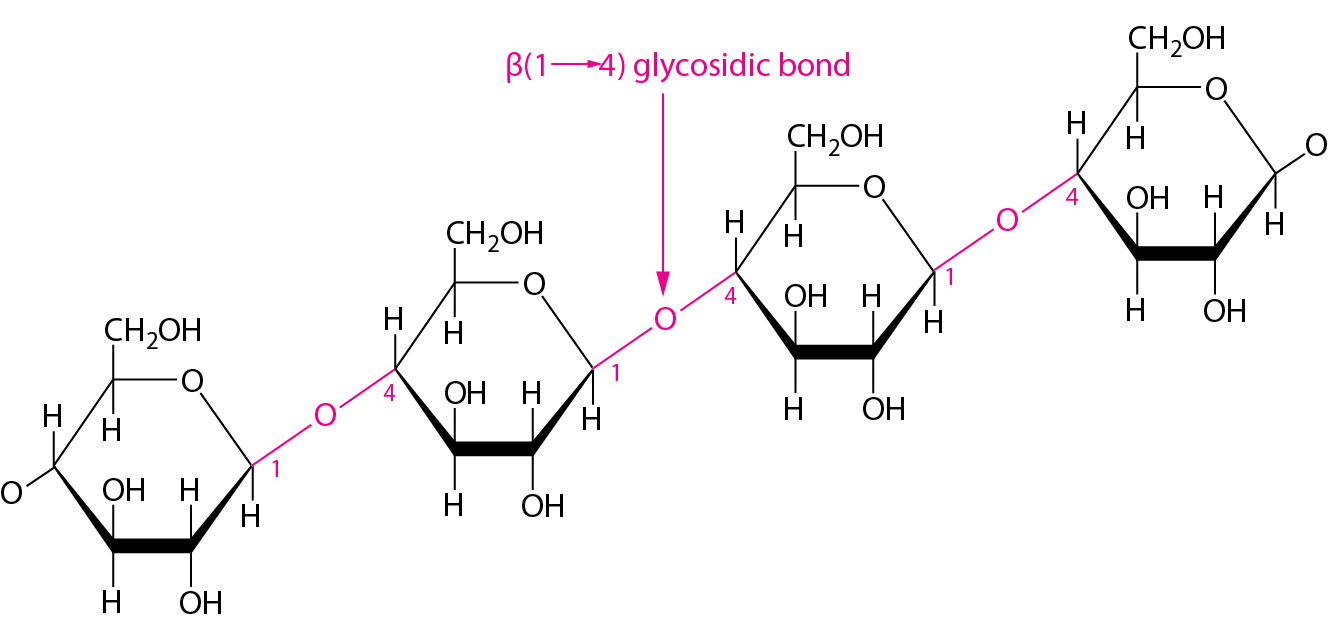
\includegraphics[width=0.7\linewidth]{Cellulose}
	\caption[Cellulose]{Cellulose}
	\label{fig:cellulose}
\end{figure}

\section{Lipiden}
\begin{figure}[htbp]
	\centering
	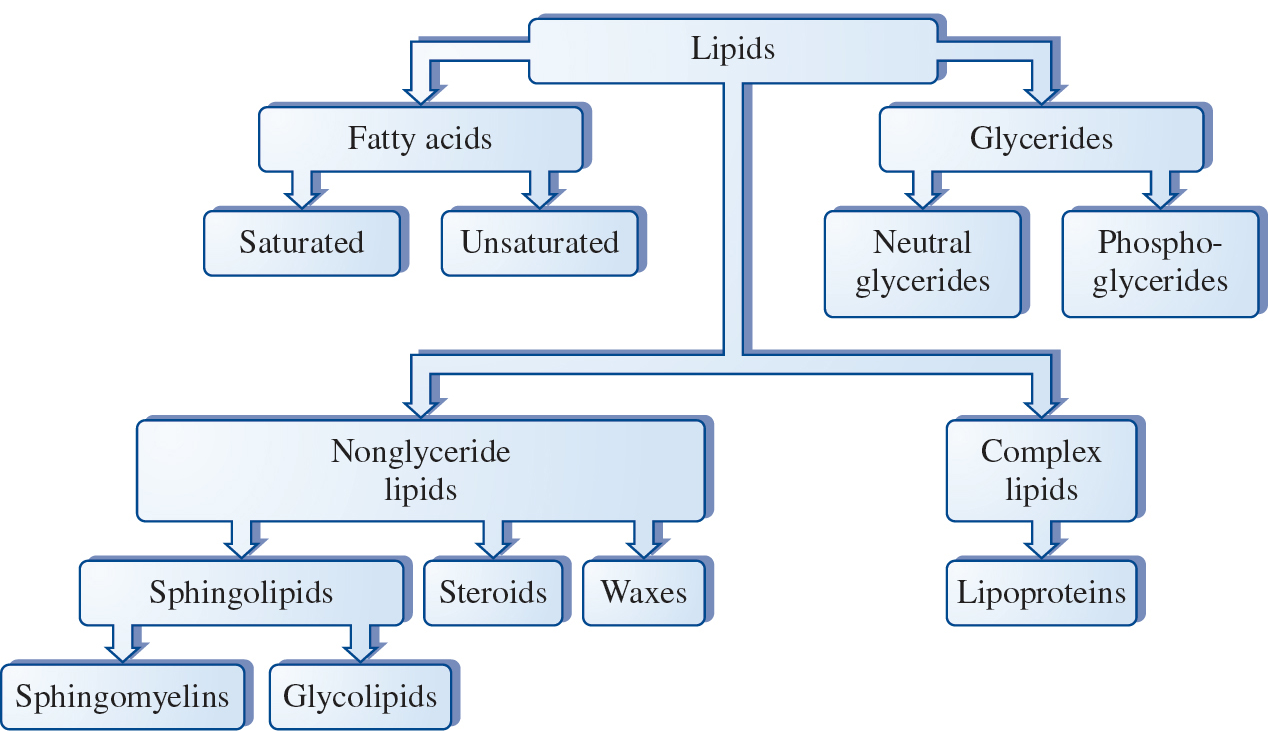
\includegraphics[width=0.7\linewidth]{Schema_lipiden}
	\caption[Lipiden]{Schema van lipiden}
	\label{fig:schemalipiden}
\end{figure}

%Overzicht Schema slide 28
\subsection{Biologische functies van lipiden}
Biologisch gezien zijn vetten extreem belangrijk. De mens gebruikt ze namelijk voor verschillende doeleinden:
\begin{itemize}
	\item Energiebron en -opslag
	\item Structurele componenten van het celmembraan
	\item Hormonen
	\item Vitaminen en vitamine-adsorptie
	\item Bescherming
	\item Isolatie
\end{itemize}
\subsection{Vetzuren}
\subsubsection{Structuur}
Vetzuren hebben lange ketens van monocarboxylzuren (-COOH) met een even aantal koolstofatomen (zie figuur \ref{fig:structuurvetzuur}).
\begin{figure}[h]
	\centering
	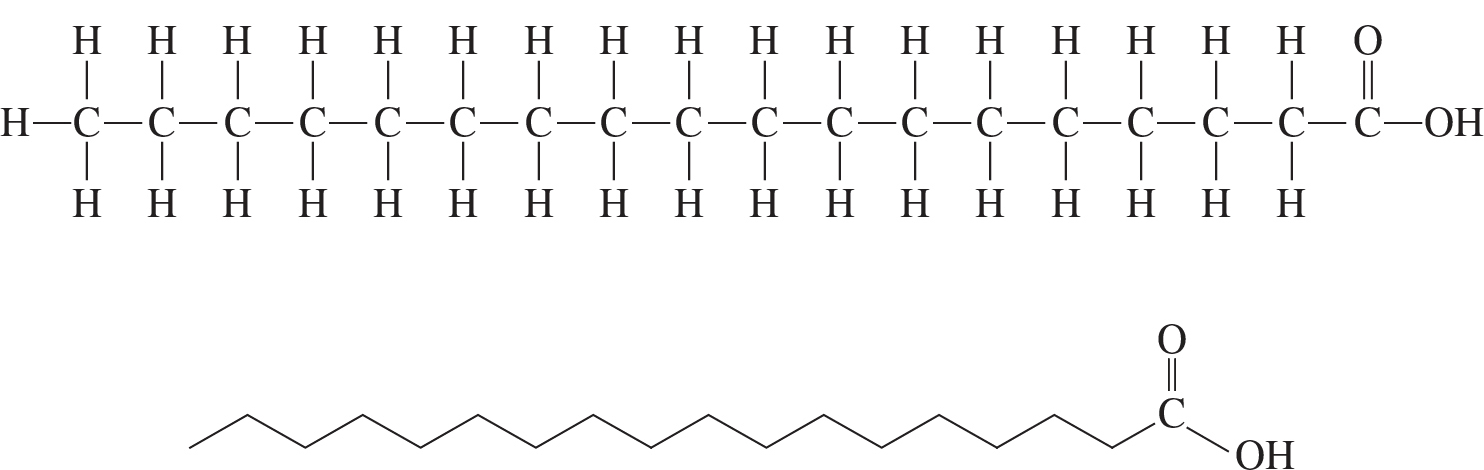
\includegraphics[width=0.7\linewidth]{StructuurVetZuur}
	\caption[Vetzuur]{Structuur van een vetzuur}
	\label{fig:structuurvetzuur}
\end{figure}
\subsubsection{(On)Verzadigde vetzuren}
Verzadigde vetzuren bestaan uitsluitend uit enkelvoudig gebonden koolstof atomen zoals in figuur \ref{fig:structuurvetzuur}. We spreken van een onverzadigd vetzuur als er een dubbele binding voorkomt tussen de koolstoffen zoals in figuur \ref{fig:onverzadigdevetzuren}.
\begin{figure}[h]
	\centering
	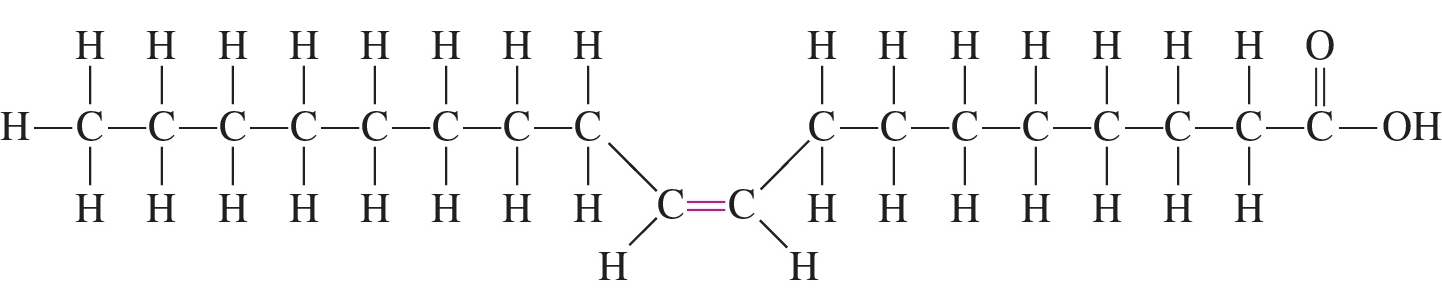
\includegraphics[width=0.7\linewidth]{OnVerzadigdeVetzuren}
	\caption[Onverzadigde VZ]{Onverzadigde vetzuren}
	\label{fig:onverzadigdevetzuren}
\end{figure}\\
We vinden verzadigde vetzuren vaak bij dieren en onverzadigde vetzuren bij planten. Ook het smeltpunt kent grote verschillen tussen beide soorten (zie figuur \ref{fig:smeltpuntvetzuren}). Grosso modo kunnen we zeggen dat het smeltpunt van verzadigde vetzuren afhangt van de lengte van de koolstofketen (London krachten). Bij onverzadigde vetzuren is het smeltpunt invers proportioneel aan het aantal onverzadigde bindingen. 
\begin{figure}[h]
	\centering
	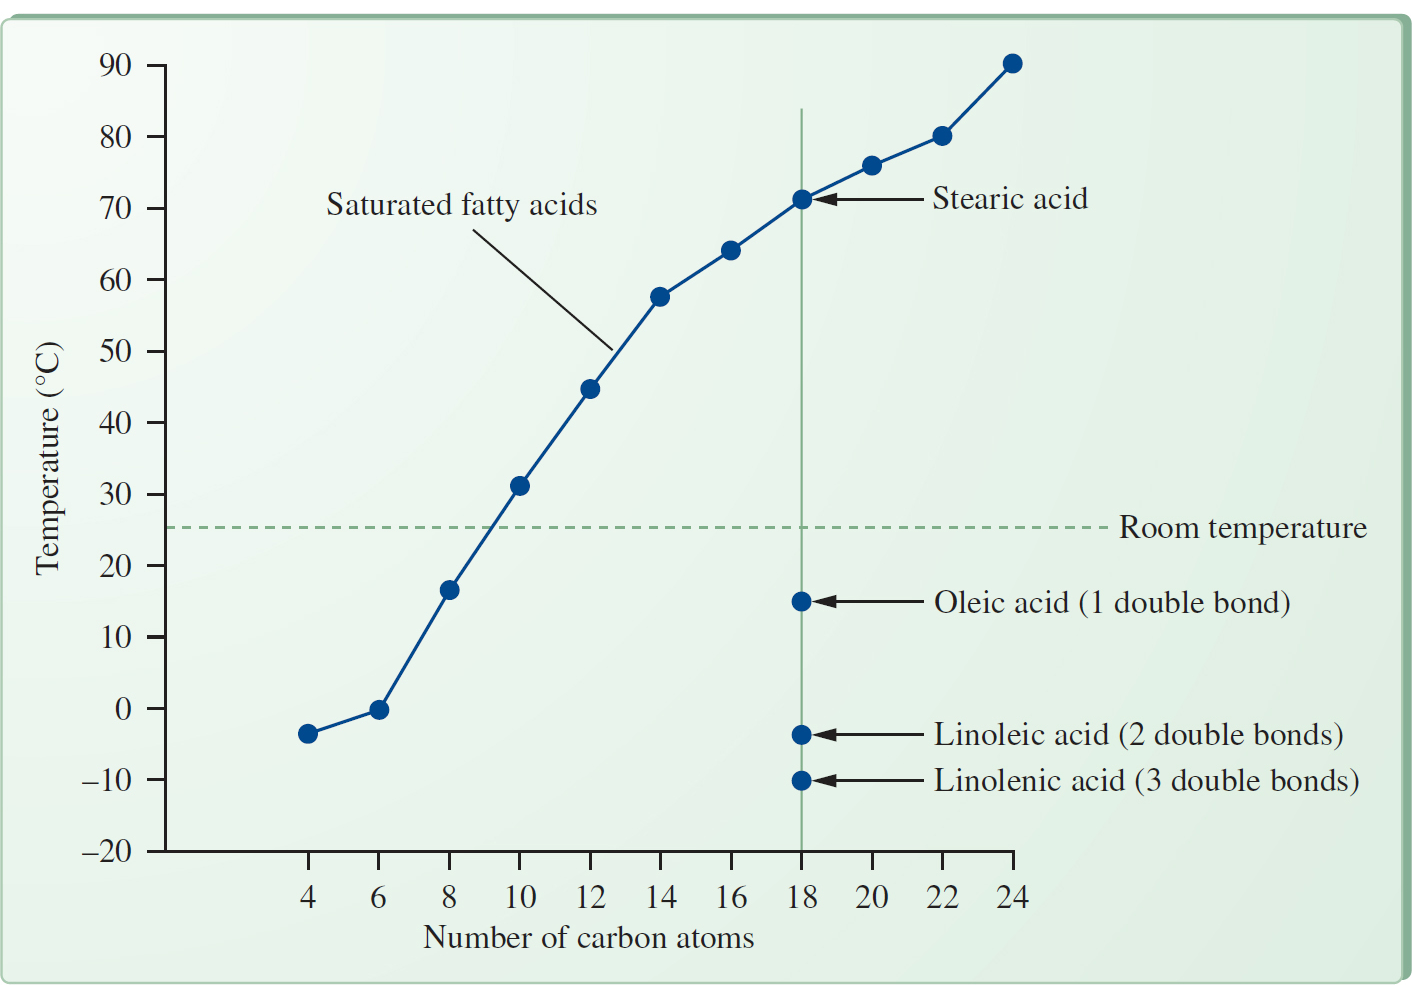
\includegraphics[width=0.7\linewidth]{smeltpuntVetzuren}
	\caption[Smeltpunt]{Smeltpunt van verzadigde en onverzadigde vetzuren}
	\label{fig:smeltpuntvetzuren}
\end{figure}
\subsubsection{Cis- en Transvetzuren}
Het verschil tussen cis- en transvetzuren zit in de manier waarop de koolstof atomen onderling georiënteerd zijn (zie figuur \ref{fig:cistransvz}). Over het algemeen kunnen we zeggen dat Transvetzuren slecht zijn voor de mens, ze hebben een negatief effect op zaken zoals cholesterol en hart- en vaatziekten. We vinden ze vaak bij producten gemaakt van herkauwers, en na verhitting van vetzuren. Cisvetzuren daarentegen hebben een positieve invloed op cholesterol.
\begin{figure}[h]
	\centering
	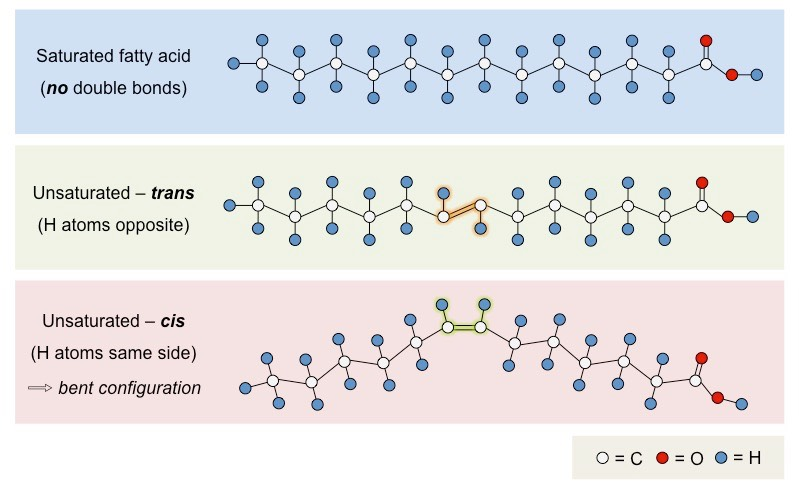
\includegraphics[width=0.7\linewidth]{CisTransVZ}
	\caption[Cis en Trans]{Cis- en Transvetzuren}
	\label{fig:cistransvz}
\end{figure}
\newpage
\subsubsection{Omega vetzuren}
We spreken hoofdzakelijk over Omega 3 en omega 6 vetzuren. Het zijn onverzadigde vetzuren die hun naam krijgen op basis van het aantal verzadigde bindingen voor de eerste dubbele binding, zie figuur \ref{fig:omegaVZ}. 
\begin{figure}[h]
	\centering
	\begin{subfigure}{.5\textwidth}
		\centering
		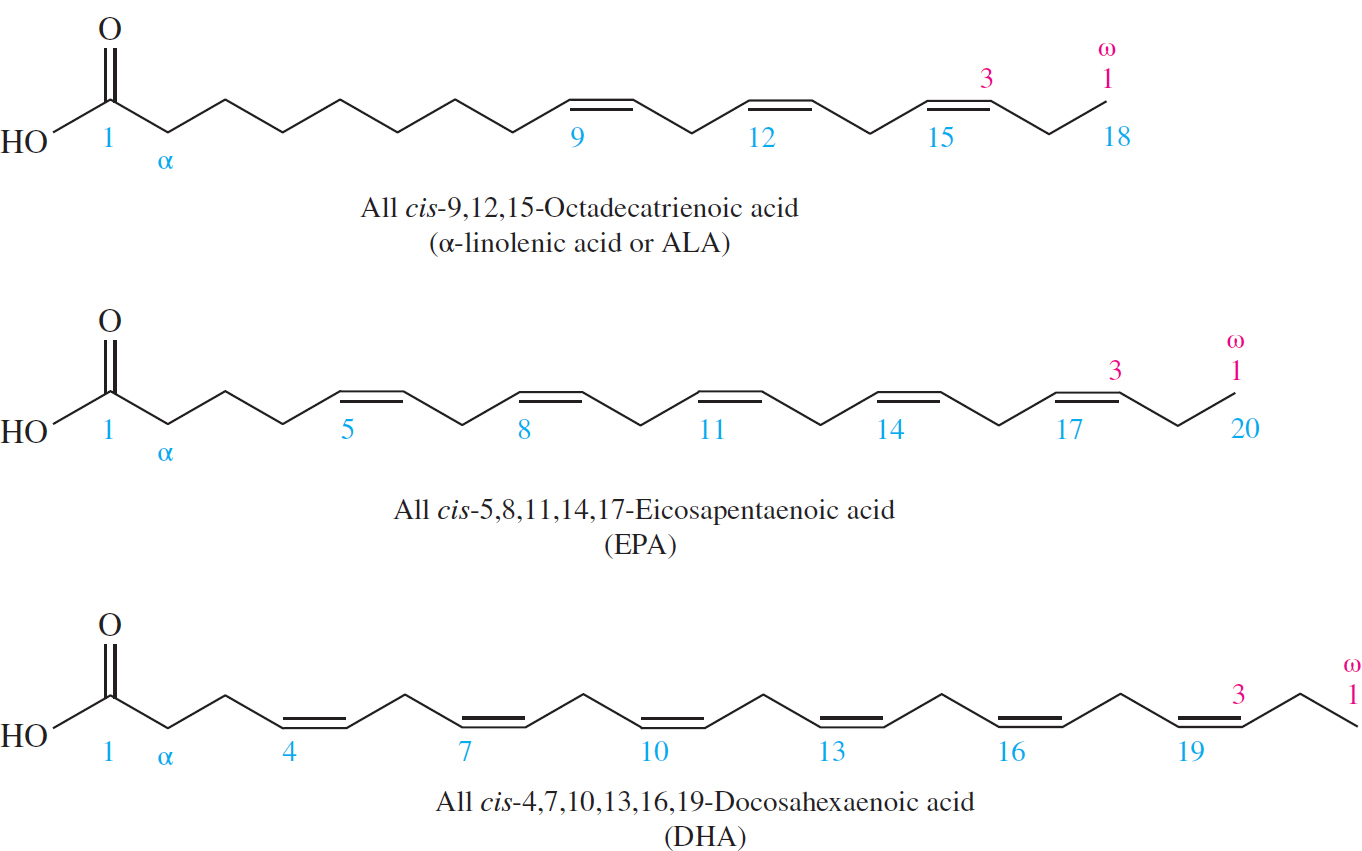
\includegraphics[width=1\linewidth]{Omega3VZ}
		\caption{Omega 3 vetzuur}
		\label{fig:Omega3}
	\end{subfigure}%
	\begin{subfigure}{.5\textwidth}
		\centering
		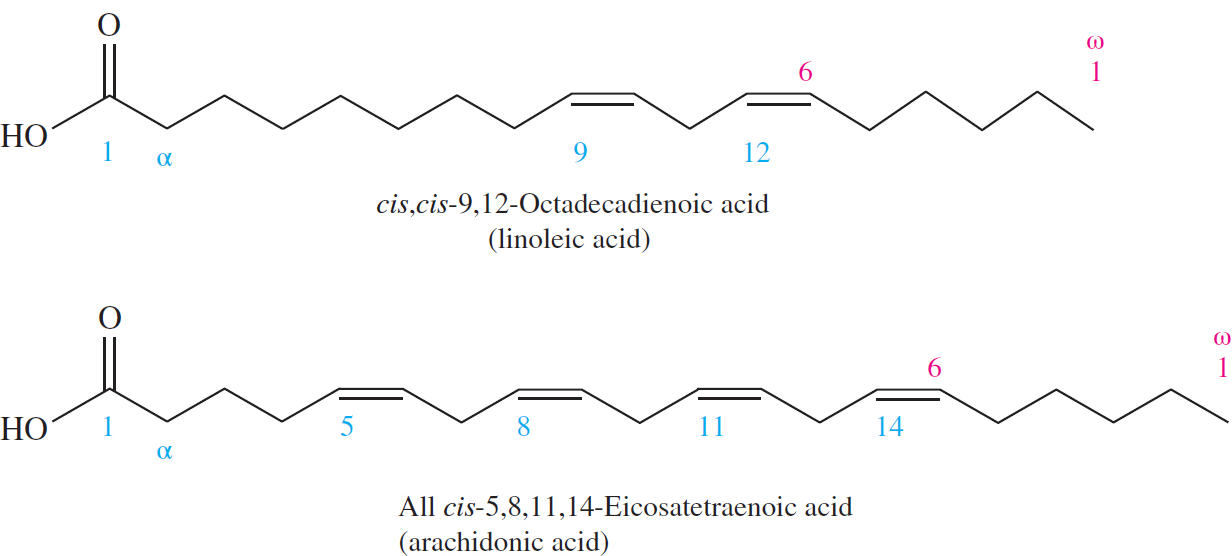
\includegraphics[width=1\linewidth]{Omega6VZ}
		\caption{Omega 6 vetzuur}
		\label{fig:Omega6}
	\end{subfigure}
	\caption{Het verschil tussen veel en weinig vertakkingen}
	\label{fig:omegaVZ}
\end{figure}\\
We associëren omega 3 vetzuren vaak met positieve gezondheidseffecten, onderzoek wijst namelijk uit dat het hart- en vaatziekten tegenhoud en een ontstekingsremmend effect heeft. Omega 6 vetzuren komen met ongewenste gezondheidseffecten.
\subsubsection{Reacties met vetzuren}
De belangrijkste reactie voor deze cursus is de hydrogenering (zie figuur ). Het is een additie reactie waarbij onverzadigde vetzuren omgezet worden in verzadigde vetzuren. Deze reactie wordt sterk gebruikt in de voedingsindustrie.
\begin{figure}[h]
	\centering
	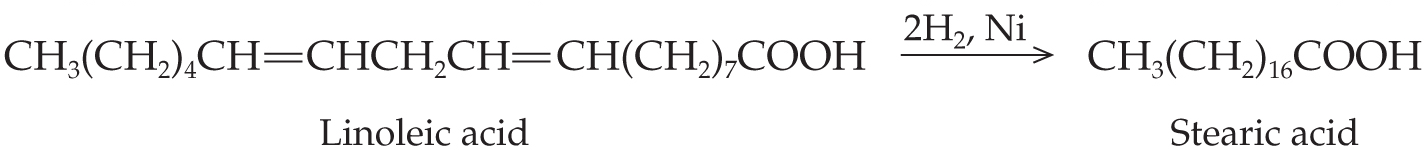
\includegraphics[width=0.7\linewidth]{hydrogenering}
	\caption[Hydrogenering]{Hydrogenering}
	\label{fig:hydrogenering}
\end{figure}
%Mooie samenvatting op slide 16
\subsection{Glyceriden}
\subsubsection{Structuur}
Glyceriden zijn lipide-esters, dit wil zeggen dat de alcoholgroep van glycerol een ester vormt met een vetzuur (zie figuur \ref{fig:structuurglyceriden}). Deze estervorming kan zich op één, twee of alle 3 de alcoholgroepen van de glycerol voordoen. We spreken van mono-, di-, triglyceriden.
\begin{figure}[h]
	\centering
	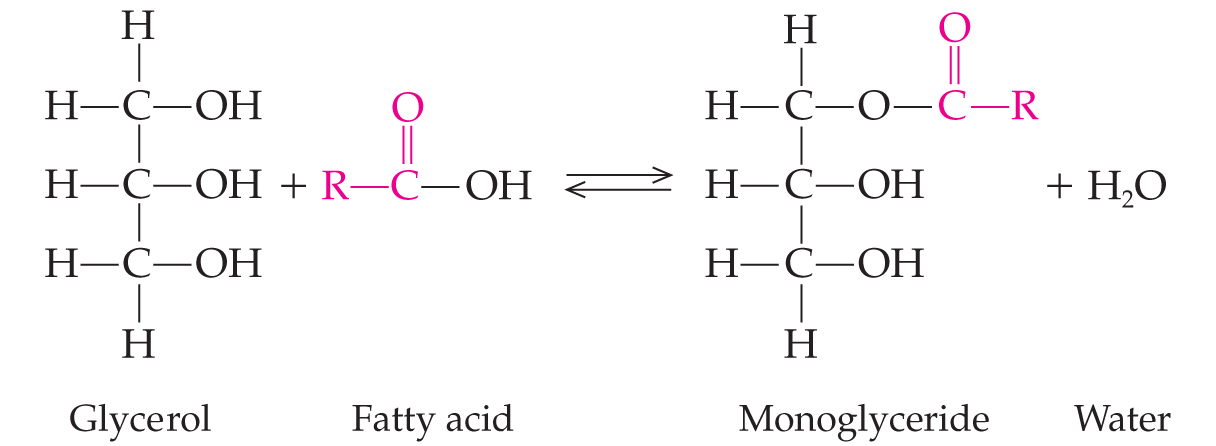
\includegraphics[width=0.6\linewidth]{structuur_glyceriden}
	\caption[Structuur glyceriden]{Structuur glyceriden}
	\label{fig:structuurglyceriden}
\end{figure}

\subsubsection{Triglyceriden}
Triglyceriden zijn non-ionische en niet polaire moleculen (zie figuur \ref{fig:triglyceride}) die dienen als energieopslag in vetcellen. Het zijn de meest voorkomende neutrale glyceriden in de natuur. Ze zijn bij vissen en planten vloeibaar bij kamertemperatuur dankzij de grote hoeveelheid onverzadigde vetzuren die aanwezig zijn. Bij mens en dier zijn de vetzuren hoofdzakelijk verzadigd, en dus zijn de triglyceriden ook vast bij kamertemperatuur.
\begin{figure}[h]
	\centering
	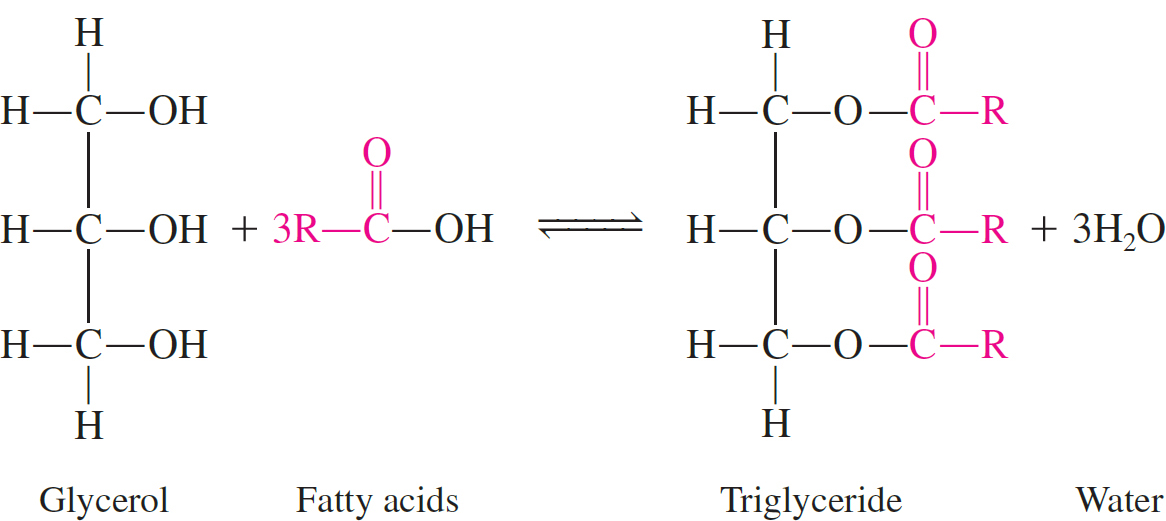
\includegraphics[width=0.6\linewidth]{Triglyceride}
	\caption[Triglyceride]{Triglyceride}
	\label{fig:triglyceride}
\end{figure}
\subsubsection{Reacties}
\textbf{Hydrolyse}\\
Produceert de vetzuren en glycerol. Het breekt dus eigenlijk een mono-, di-, triglyceride af tot zijn basiscomponenten (zie figuur \ref{fig:hydrolyseglyceriden}).
\begin{figure}[h]
	\centering
	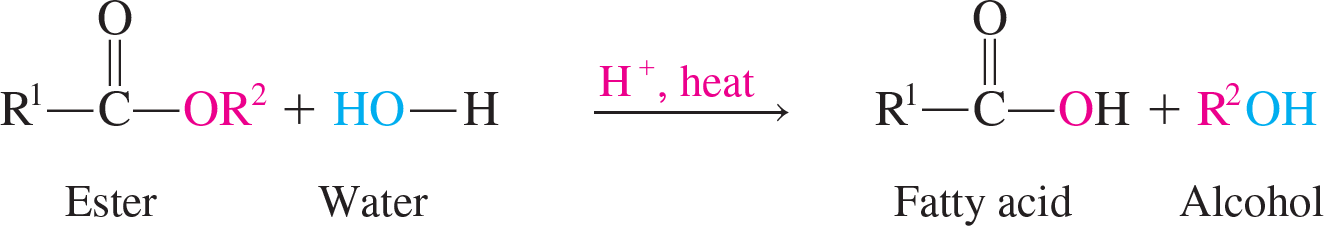
\includegraphics[width=0.7\linewidth]{HydrolyseGlyceriden}
	\caption[Hydrolyse]{Hydrolyse}
	\label{fig:hydrolyseglyceriden}
\end{figure}\\
\textbf{Verzeping}\\
Produceert vetzuurzouten en glycerol (zie figuur \ref{fig:verzepingglyceriden}).
\begin{figure}[h]
	\centering
	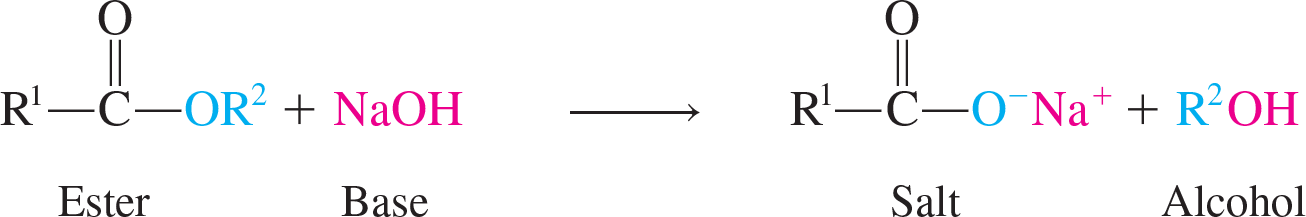
\includegraphics[width=0.7\linewidth]{VerzepingGlyceriden}
	\caption[Verzeping]{Verzeping}
	\label{fig:verzepingglyceriden}
\end{figure}
 \newpage
\subsubsection{Fosfoglyceriden}
Fosfoglyceriden zijn niet-neutrale glyceriden die opgemaakt zijn uit glycerol, vetzuur en een fosfaat-groep waarop eventueel nog andere groepen gebonden zijn zoals in figuur \ref{fig:fosfoglyeride}. De functie ervan zal later aan bod komen in het hoofdstuk over cellen. 
\begin{figure}[h]
	\centering
	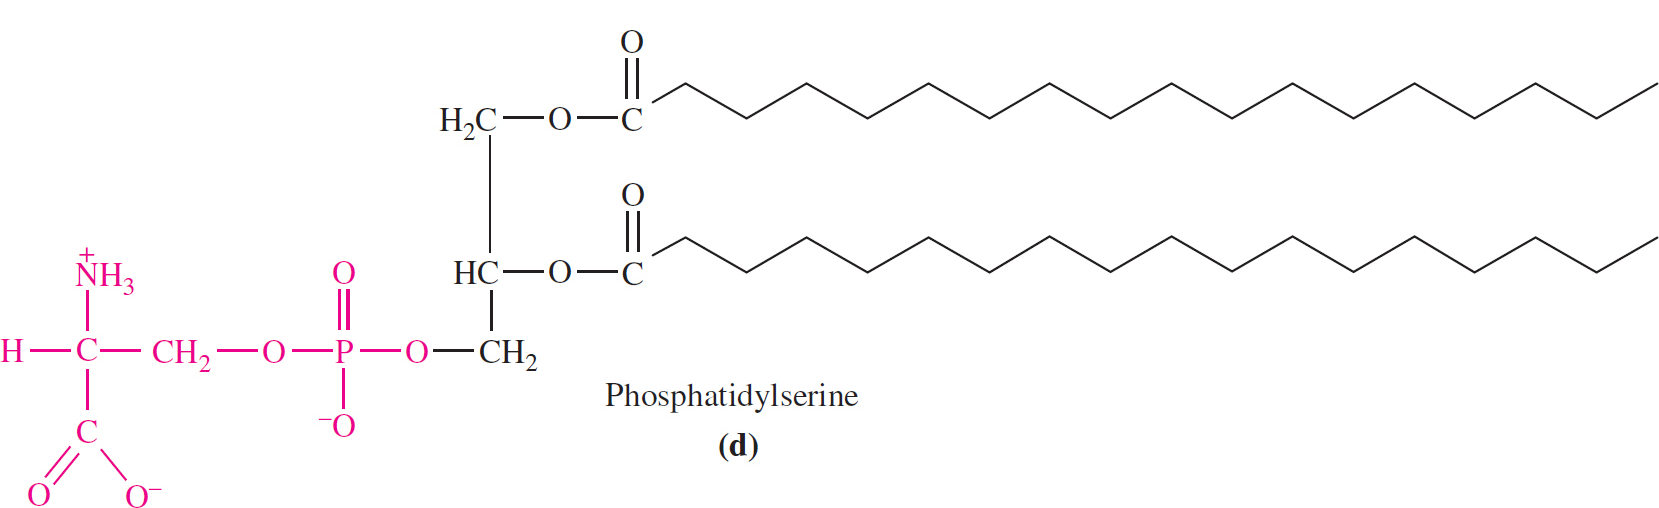
\includegraphics[width=0.7\linewidth]{fosfoglyeride}
	\caption[Fosfoglyceride]{Fosfoglyceride}
	\label{fig:fosfoglyeride}
\end{figure}

\subsection{Niet-glyceride lipiden}
\subsubsection{Sfingolipide}
Sfingolipiden worden getypeerd door hun sfingosine ruggengraat (zie figuur \ref{fig:sfingolipide}). Hieraan kunnen verschillende groepen binden, zoals vetzuren, fosfaat of koolhydraten. Men vind deze moleculen vooral terug in het celmembraan. 
\begin{figure}[h]
	\centering
	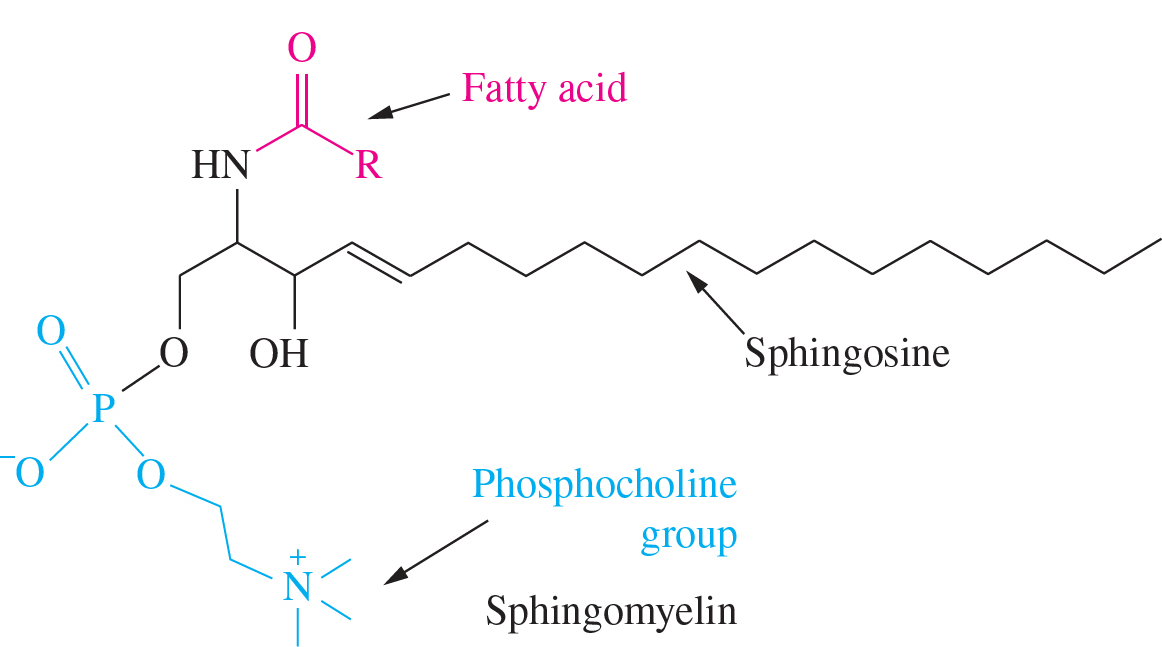
\includegraphics[width=0.5\linewidth]{sfingolipide}
	\caption[Sfingolipide]{Sfingolipide}
	\label{fig:sfingolipide}
\end{figure}
\subsubsection{Steroïden}
Steroïden volgen de algemene structuur die te zien is in figuur \ref{fig:steroidenstructuur}. 
\begin{figure}[h]
	\centering
	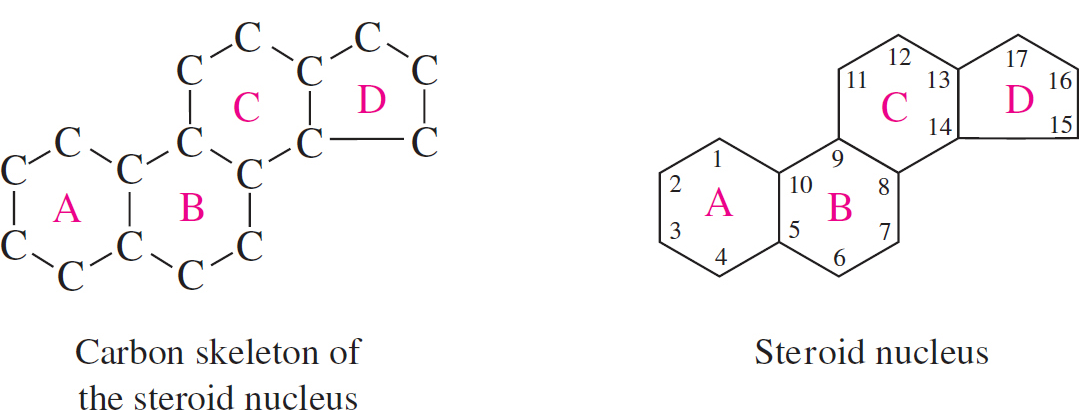
\includegraphics[width=0.5\linewidth]{steroidenstructuur}
	\caption[steroïden]{Steroïden}
	\label{fig:steroidenstructuur}
\end{figure}\\
Cholesterol is een belangrijke steroïde die we nodig hebben om galzouten, hormonen en vitaminen aan te maken. Zoals alles is een balans wel belangrijk, te veel cholesterol kan leiden tot het dichtslippen van aders. 

\section{Celstructuren}
\subsection{Microscopische observatie van cellen}
Cellen zijn bijna altijd te klein om met het blote oog te zien. Om deze levensvormen toch te zien maken we gebruik van microscopen. Hiervoor bestaan 2 technologieën: de licht microscoop en de elektronen microscoop. 

De licht microscoop is een (relatief) goedkope optie. We maken ook nog onderscheid tussen de klassieke en digitale microscoop. Door de eigenschappen van licht, is er een limiet aan de resolutie waarmee we kunnen observeren. De elektronen microscoop lost dit probleem op door een bundel elektronen te gebruiken. We kunnen opnieuw 2 verschillende soorten onderscheiden, de TEM en de SEM. 
\subsection{Celtheorie}
We stellen dat alle organismen zijn samengesteld uit cellen. Deze cellen zijn ook altijd afkomstig van reeds bestaande cellen. Cellen zijn ook klein, de reden hiervoor is de oppervlakte-volume verhouding. Dit wil zeggen dat kleine cellen een relatief grote oppervlakte hebben in vergelijking met hun volume. Aangezien cellen hun wand gebruiken voor het uitwisselen van stoffen, is het dus voordelig om een relatief groot wand oppervlak te hebben. Er zijn nog andere mogelijkheden om de oppervlakte te vergroten, zo maken enkele cellen microvilli aan zoals te zien in figuur \ref{fig:microvilli}.
\begin{figure}[h]
	\centering
	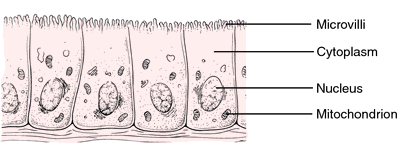
\includegraphics[width=0.7\linewidth]{Microvilli}
	\caption[Microvilli]{Microvilli}
	\label{fig:microvilli}
\end{figure}
\newpage
\subsection{Plasmamembraan}
Het Plasmamembraan markeert de grens tussen buiten en binnen een cel. Het is essentieel voor transport van stoffen in en uit de cel. Een plasmamembraan is opgebouwd uit een fosfolipide dubbellaag met ingebouwde eiwitten. Hierbij is de polaire (en dus hydrofiele) zijde van de fosfolipiden gericht naar het waterig medium. De niet-polaire staarten (hydrofoob) staan tegenover elkaar (zie figuur \ref{fig:plasmamembraan}). Als geheel vormen ze ook een vloeistofmozaïekmodel. Dit model zorgt ervoor dat het membraan extreem flexibel is. 
\begin{figure}[h]
	\centering
	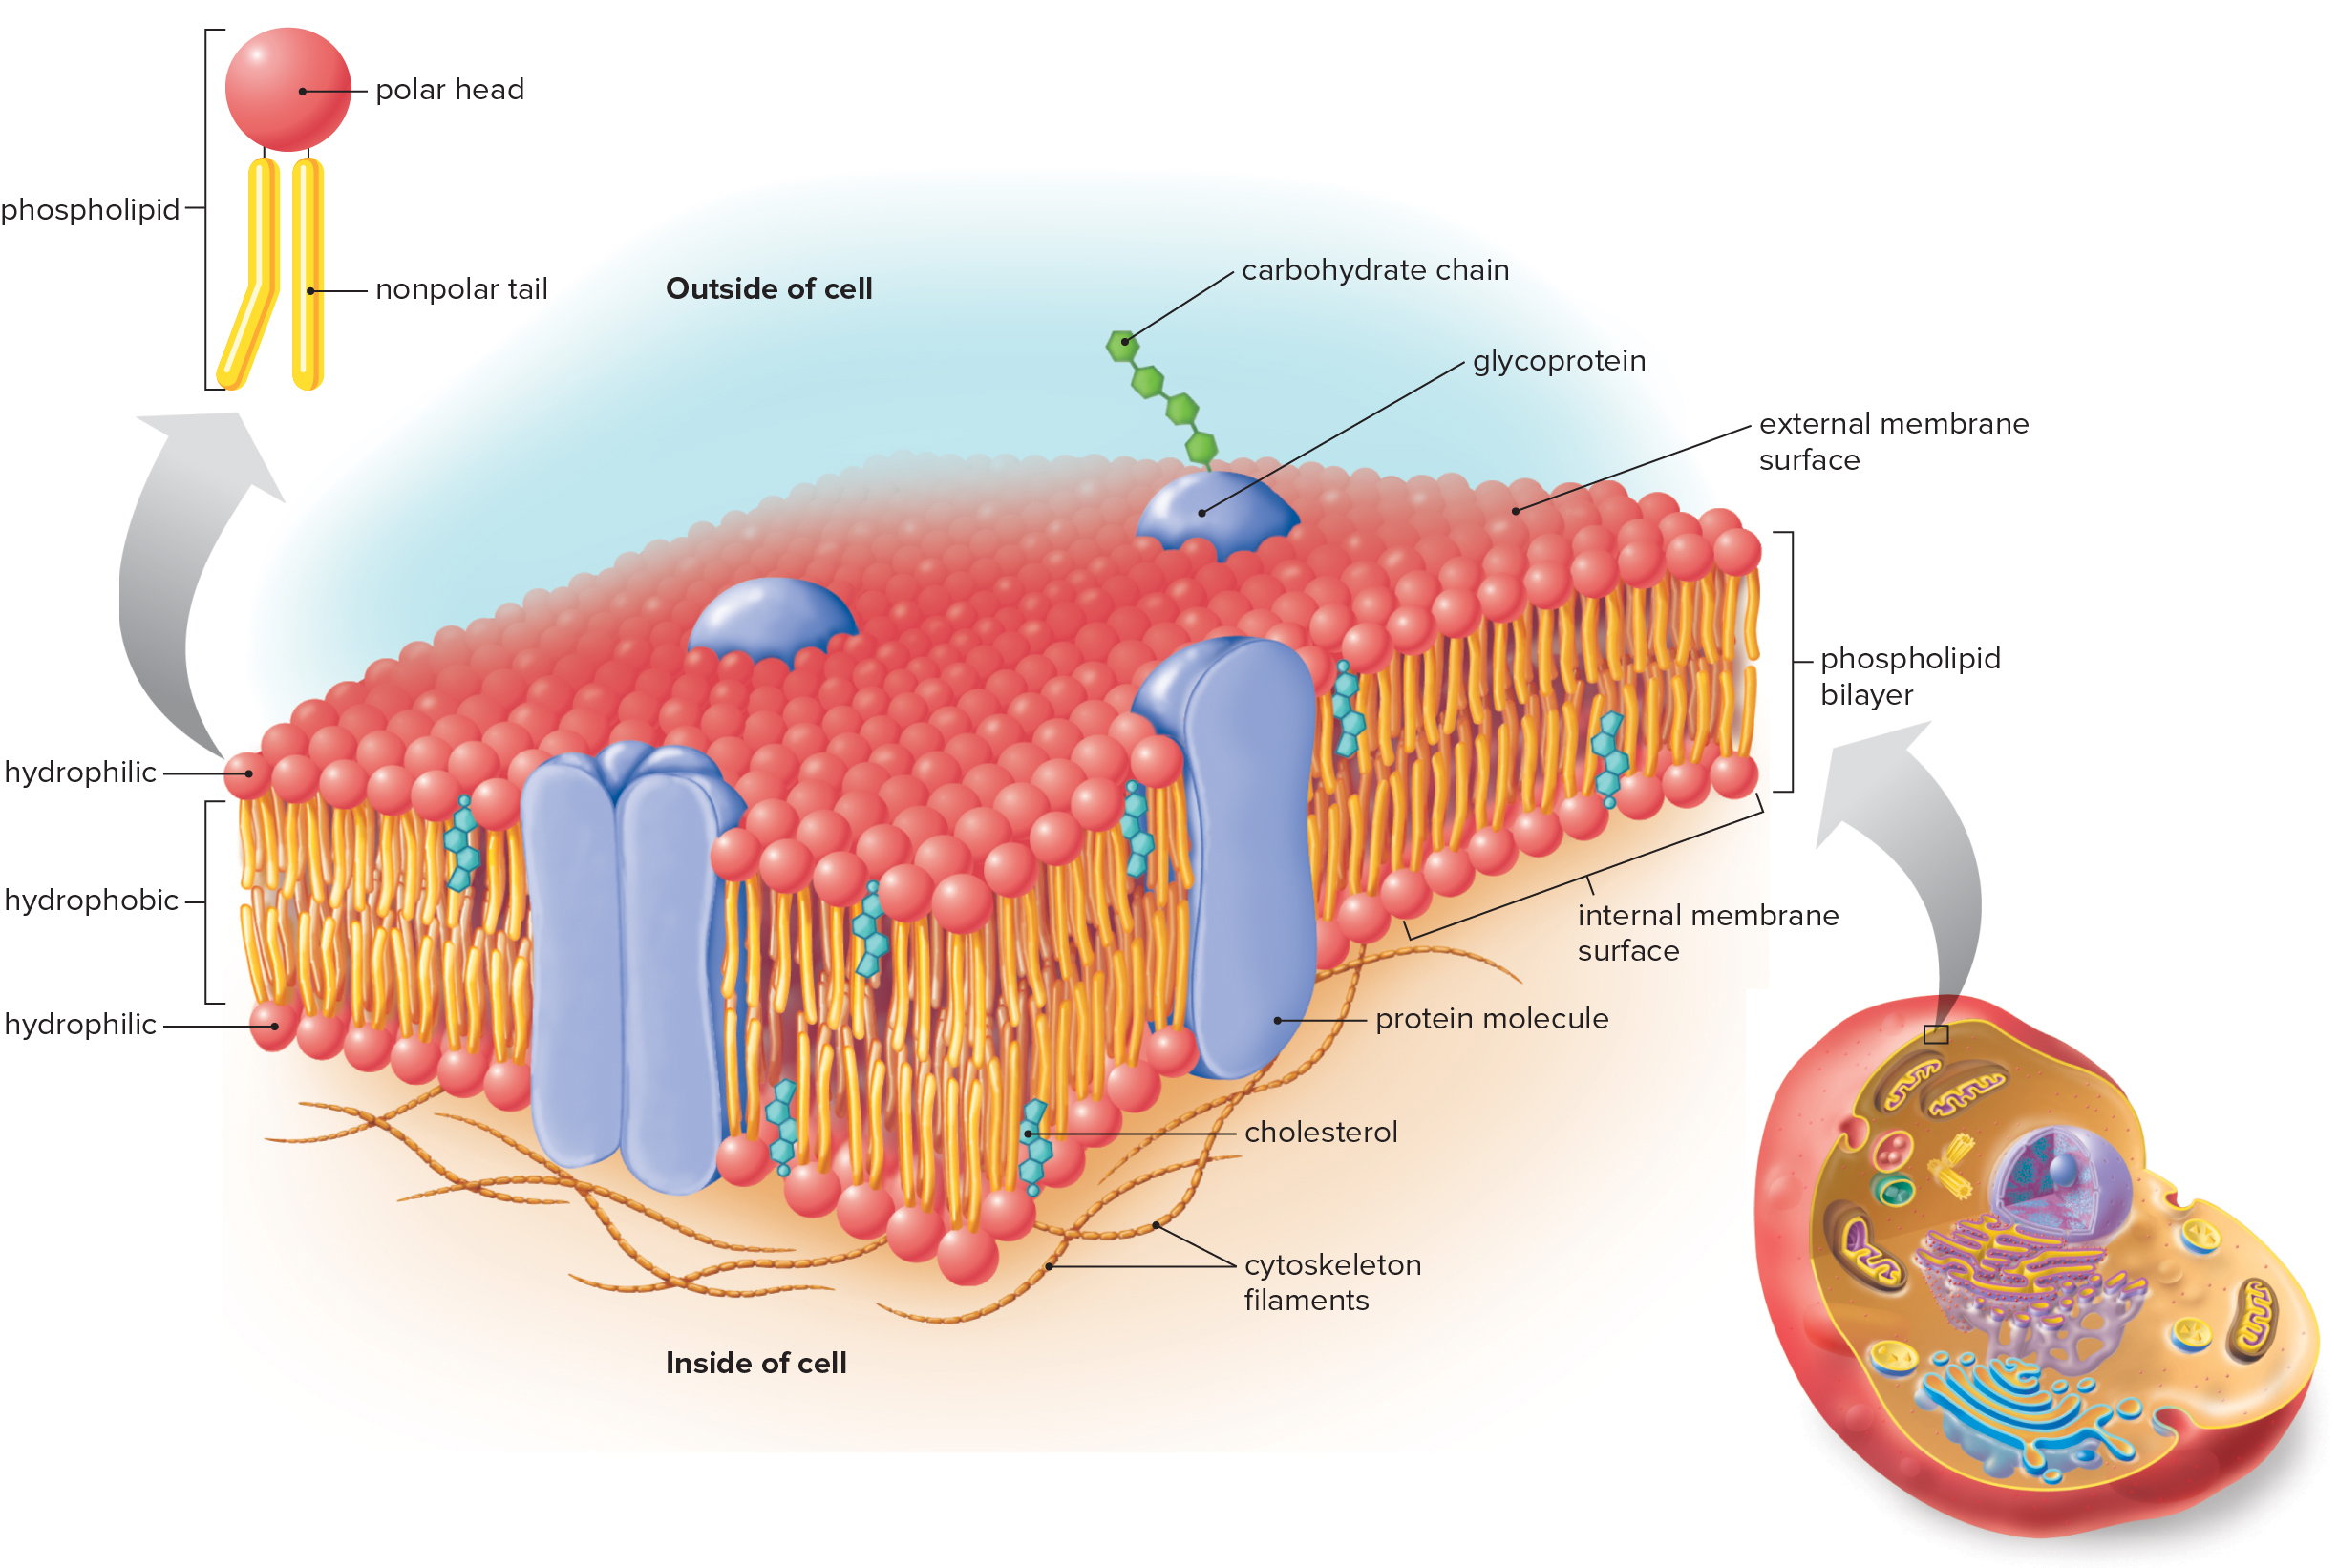
\includegraphics[width=0.8\linewidth]{Plasmamembraan}
	\caption[Plasmamembraan]{Plasmamembraan}
	\label{fig:plasmamembraan}
\end{figure}

Afhankelijk van de omstandigheden waarin de cel zich bevindt, kan de structuur van de vetzuren veranderen. In koude klimaten zullen er meer onverzadigde vetzuren aanwezig zijn, hierdoor dal de vloeibaarheid van het membraan stijgen. Het omgekeerde geldt voor cellen in warme omstandigheden. 

Membraan proteïnen zijn niet alleen belangrijk voor de communicatie van de cel, maar ook voor nutriëntenopname en afvalverwijdering. We onderscheiden 6 verschillende soorten proteïnen. Kanaalproteïnen (figuur \ref{fig:kanaal}) worden hoofdzakelijk gebruikt om specifieke moleculen door de celmembraan te loodsen; transportproteïnen (figuur \ref{fig:transport})zijn dan weer betrokken bij de doorgang van moleculen door het membraan, waarbij soms input van energie nodig is. Celherkenningsproteïnen worden gebruikt om een onderscheid te maken tussen cellen van ons eigen lichaam, en die van andere organismen (figuur \ref{fig:Celherkenningsproteïnen}). Receptorproteïnen laten signaalmoleculen toe om te binden, hierdoor ontstaat een cellulaire respons (figuur \ref{fig:Receptorproteïnen}). Enzymatische proteïnen katalyseren metabole reacties (figuur \ref{fig:Enzymproteïnen}). Tot slot worden junctie-proteïnen gebruikt om verbindingen te vormen tussen cellen, hierbij is cel-tot-cel hechting en communicatie mogelijk (figuur \ref{fig:Junctieproteïnen}).
\begin{figure}[!htbp]
	\centering
	\begin{subfigure}{.5\textwidth}
		\centering
		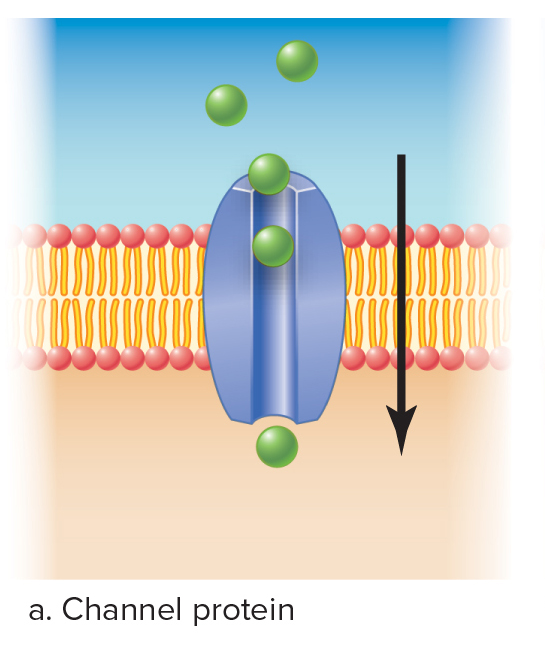
\includegraphics[width=0.7\linewidth]{Kanaalprot}
		\caption{Kanaalproteïnen}
		\label{fig:kanaal}
	\end{subfigure}%
	\begin{subfigure}{.5\textwidth}
		\centering
		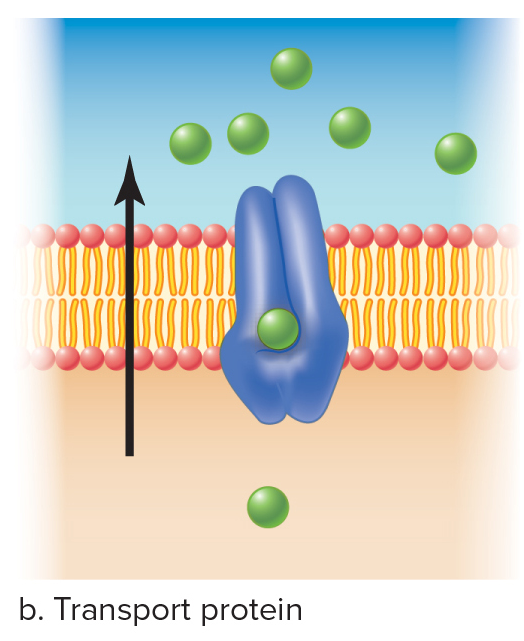
\includegraphics[width=0.7\linewidth]{transportprot}
		\caption{Transportproteïnen}
		\label{fig:transport}
	\end{subfigure}
\medskip
	\begin{subfigure}{.5\textwidth}
		\centering
		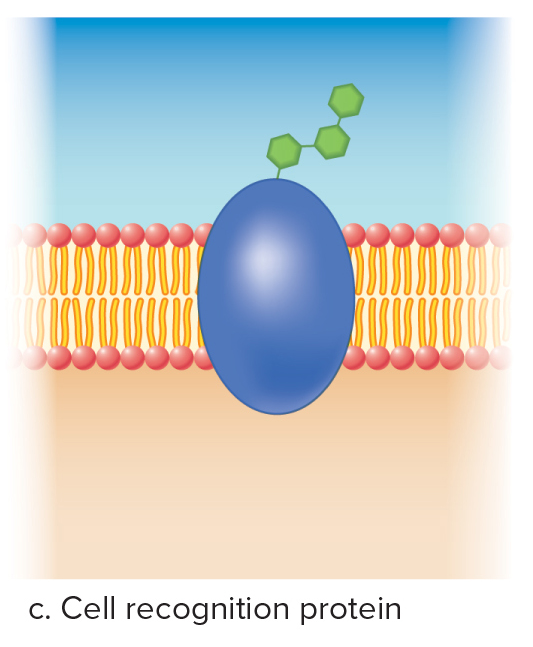
\includegraphics[width=0.7\linewidth]{Celherkenningsprot}
		\caption{Celherkenningsproteïnen}
		\label{fig:Celherkenningsproteïnen}
	\end{subfigure}%
	\begin{subfigure}{.5\textwidth}
		\centering
		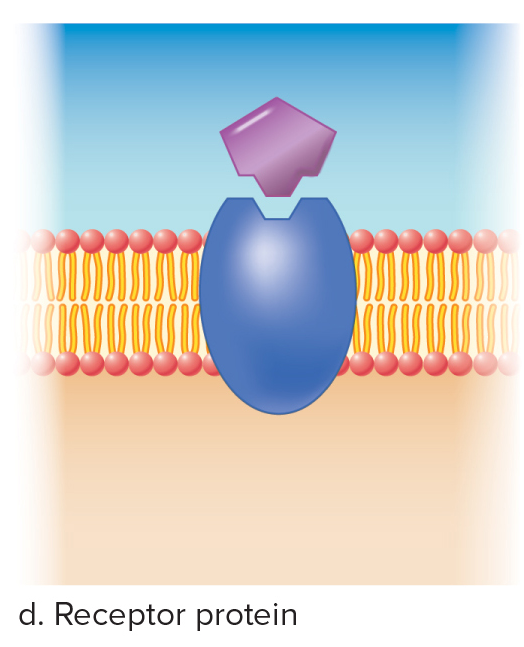
\includegraphics[width=0.7\linewidth]{Receptorprot}
		\caption{Receptorproteïnen}
		\label{fig:Receptorproteïnen}
	\end{subfigure}
\medskip
	\begin{subfigure}{.5\textwidth}
		\centering
		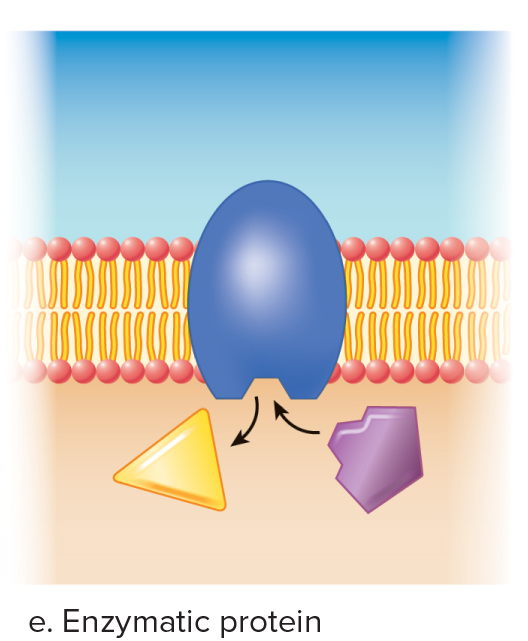
\includegraphics[width=0.7\linewidth]{Enzymatischeprot}
		\caption{Enzymatische proteïnen}
		\label{fig:Enzymproteïnen}
	\end{subfigure}%
	\begin{subfigure}{.5\textwidth}
		\centering
		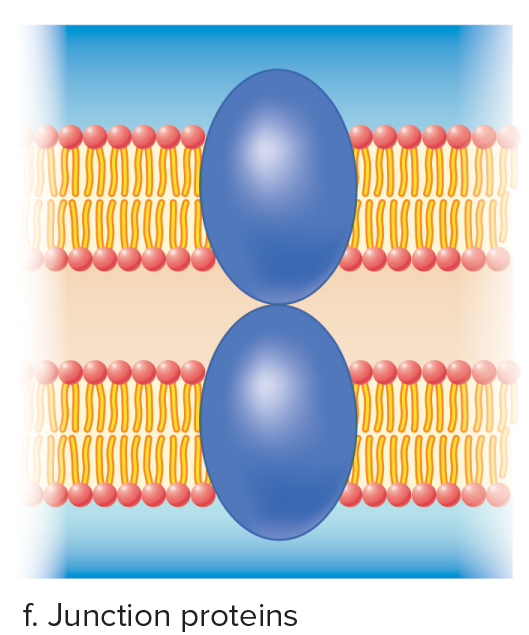
\includegraphics[width=0.7\linewidth]{Junctieprot}
		\caption{Junctie-proteïnen}
		\label{fig:Junctieproteïnen}
	\end{subfigure}
	\caption{Membraanproteïnen}
	\label{fig:membraanprot}
\end{figure}\\

\newpage
\newpage
\subsection{2 types cellen}
We definiëren twee types cellen op basis van de organisatie van genetisch materiaal. Prokaryote cellen hebben geen celkern, Eukaryote cellen hebben membraanomringd DNA.  
\subsubsection{Prokaryote cellen}
Het zijn eencellige organismen die uit de bacteria en archaea domeinen komen. Over het algemeen zijn het kleine en vrij eenvoudige organismen. Hierdoor zijn ze wel in staat om snel en effectief te reproduceren. Ze zijn hierdoor ook een zeer diverse groep organismen. 

Bacteriën zijn bekende prokaryote cellen. Ze kunnen bij de mens verschillende ziektes veroorzaken, maar ze hebben ook voordelen. We gebruiken ze om chemicaliën, voedsel en geneesmiddelen te produceren. 

De structuur van prokaryote cellen kan sterk verschillen, hier nemen we het voorbeeld van een bacterie. zoals te zien is in figuur \ref{fig:prokaryotecellen}, hebben we cytoplasma dat omringd is door een plasmamembraan en celwand. Per uitzondering kan deze celwand niet aanwezig zijn, er is ook een mogelijkheid op een beschermende capsule. De celwand is verantwoordelijk voor het behoud van de vorm van de cel.  Het cirkelvormig dubbelstrengig DNA bevindt zich in het nucleoid zonder omringend membraan. Er zijn ook andere celstructuren aanwezig die later besproken worden. 

\begin{figure}[h]
	\centering
	\includegraphics[width=0.7\linewidth]{Prokaryote_cellen}
	\caption[Prokaryote cel]{Prokaryote cel}
	\label{fig:prokaryotecellen}
\end{figure}
\newpage
\subsubsection{Eukaryote cellen}
Dit zijn vaak dierlijke cellen, ze maken dus een deel uit van een multicellulair organisme. Soms komen ze ook vaak als micro-organismen, deze kunnen multicellulair zijn, maar kunnen ook unicellulair zijn zoals bijvoorbeeld gist. Ook algen bestaan uit eukaryote cellen. In het algemeen zijn dit complexere levensvormen (zie figuur \ref{fig:eukaryotecel}). De aanwezige celstructuren worden besproken in subsectie \ref{sec:IntracellulaireStructuren}. 
\begin{figure}[h]
	\centering
	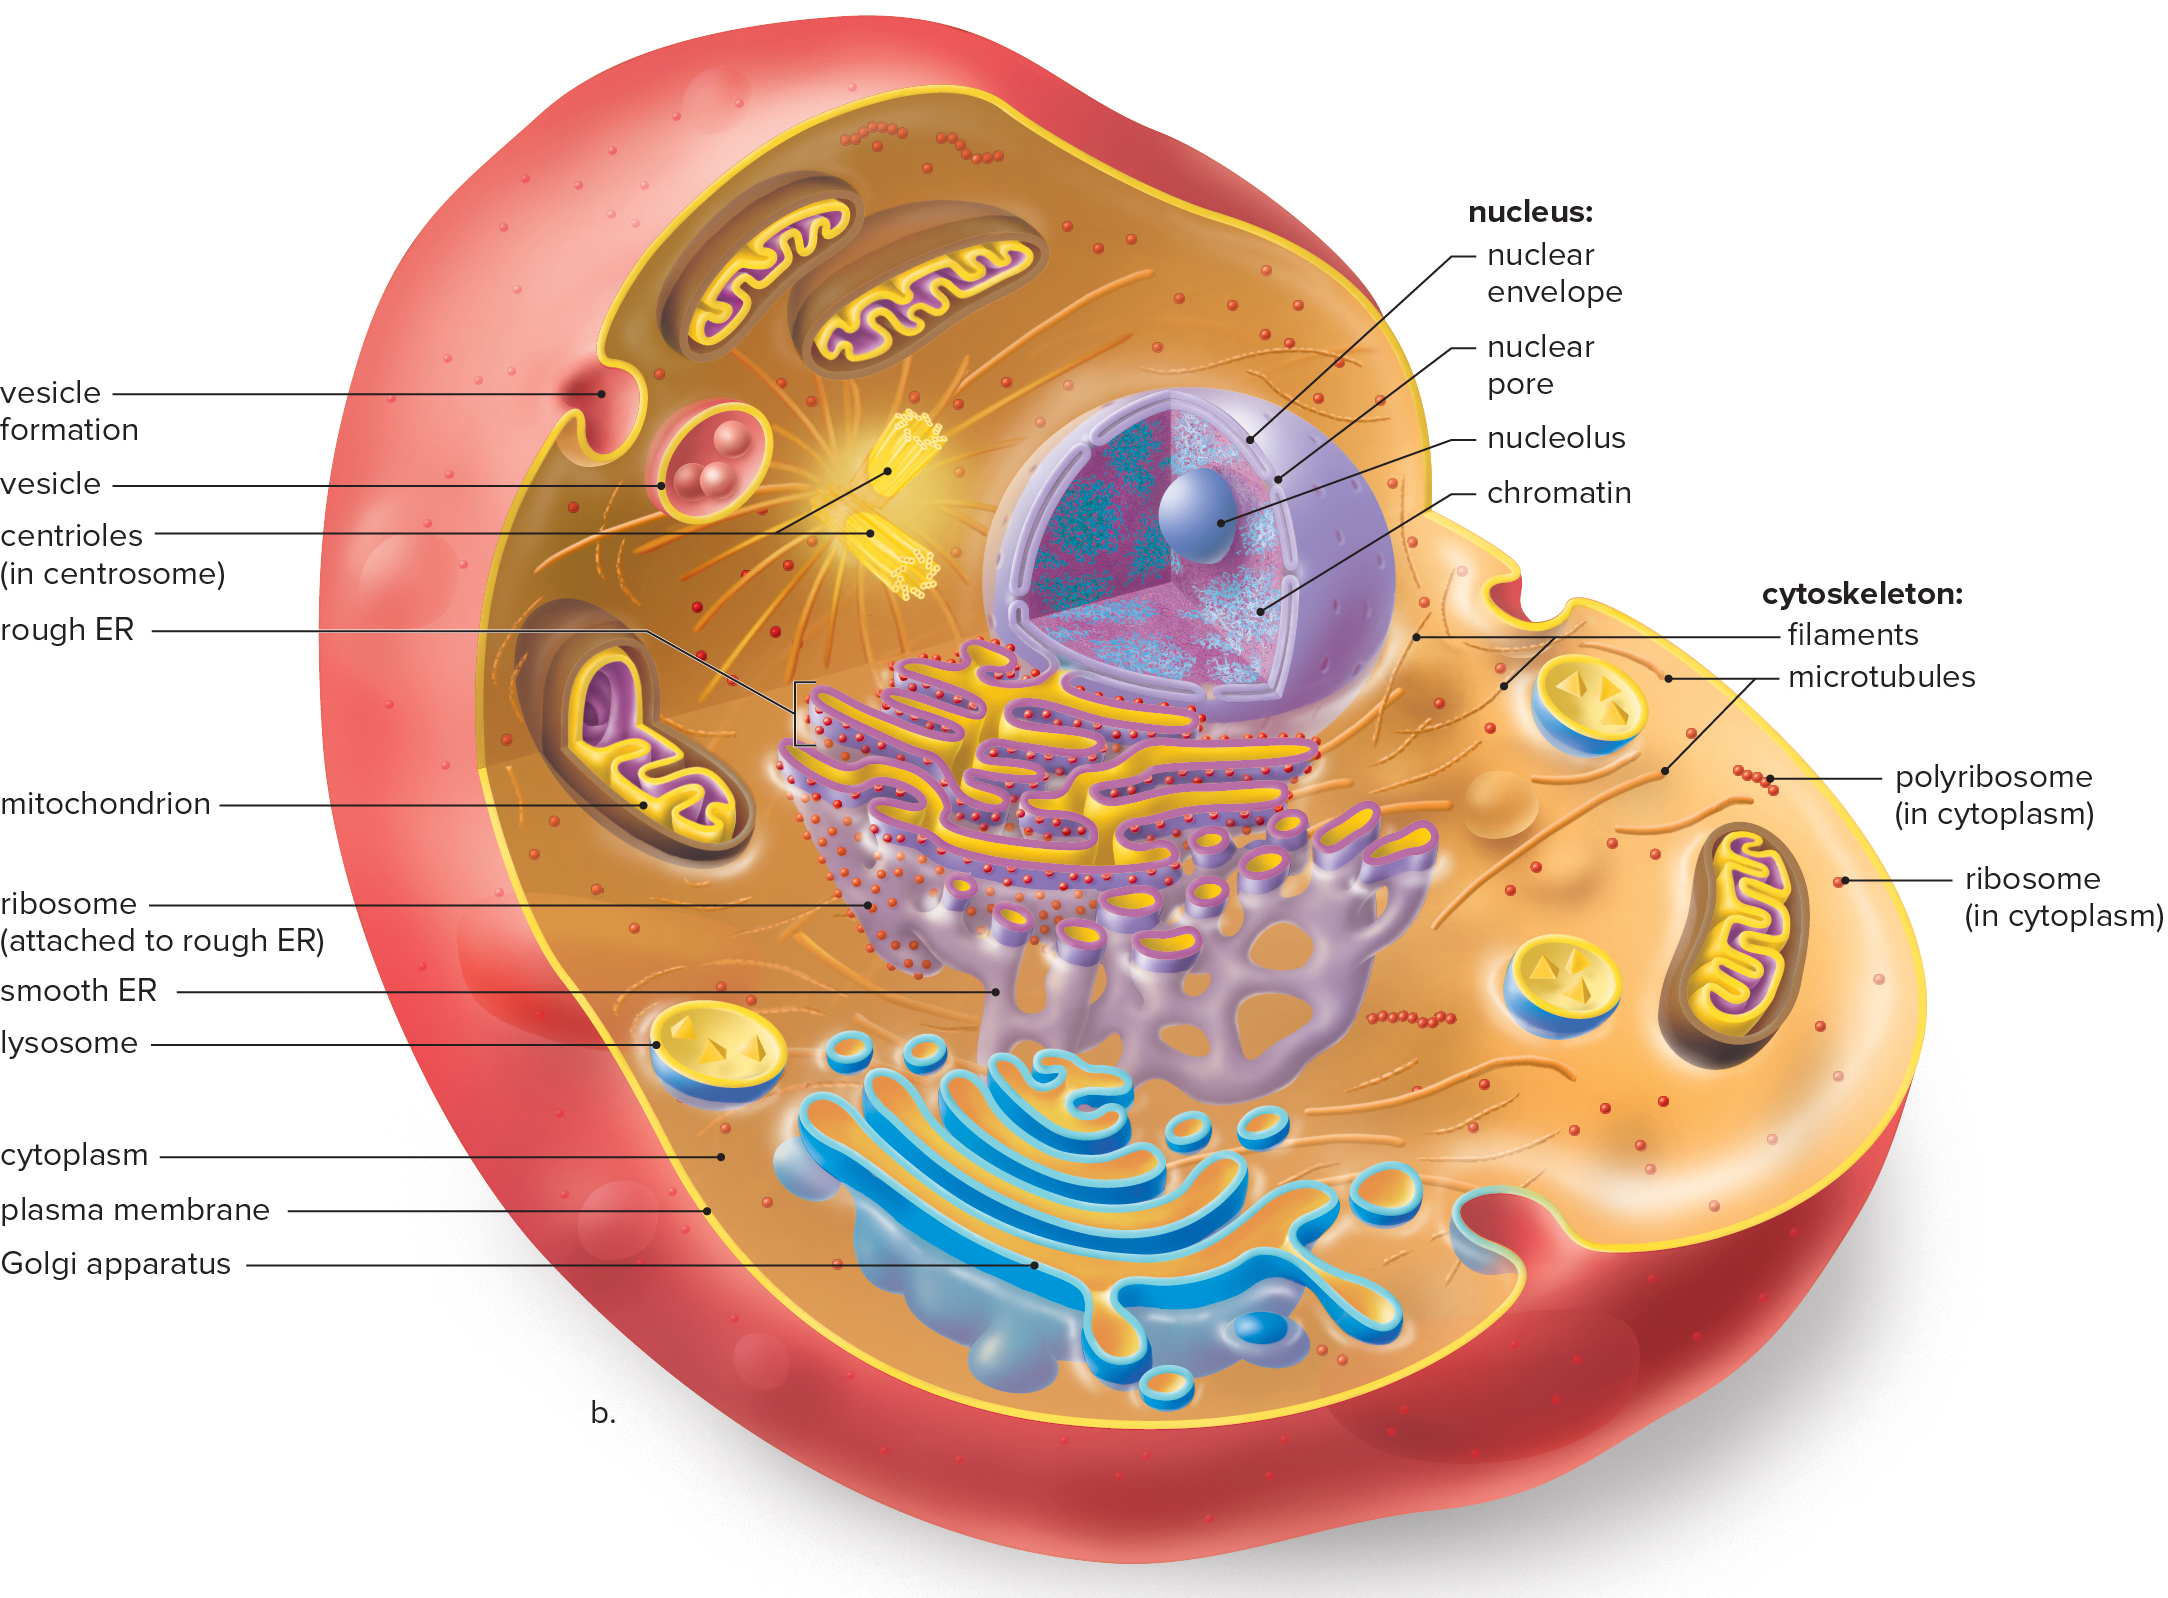
\includegraphics[width=0.5\linewidth]{Eukaryote_cel}
	\caption[Eukaryote cel]{Eukaryote cel}
	\label{fig:eukaryotecel}
\end{figure}

\subsection{Intracellulaire structuren}
\label{sec:IntracellulaireStructuren}
\subsubsection{Nucleus}
De nucleus (zie figuur \ref{fig:nucleus}) oftewel de celkern is een nucleaire envelop gemaakt uit een dubbel membraan. Nucleaire poriën zorgen voor transport van stoffen in en uit de kern. De belangrijkste taak van de celkern is om genetische informatie op te slaan. Dit gebeurt met chromatine, een soort geheel van DNA, proteïne en RNA (Voor celdeling zal het DNA zich condenseren in lineaire chromosomen). DNA met informatie in genen zal een transcriptie krijgen naar messengerRNA oftewel mRNA. Dit proces gebeurt buiten de celkern in het cytoplasma, met behulp van ribosomen wordt mRNA dan vertaald in polypeptiden. De Nucleolus is de regio waar ribosomaalRNA oftewel rRNA wordt aangemaakt.
\begin{figure}[h]
	\centering
	\includegraphics[width=0.5\linewidth]{Nucleus}
	\caption[Nucleus]{Nucleus}
	\label{fig:nucleus}
\end{figure}

\subsubsection{Ribosomen}
Ribosomen (figuur \ref{fig:ribosoom}) zijn verantwoordelijk voor de eiwitsynthese, dit gebeurt in het cytoplasma. We vinden deze structuur in zowel prokaryote als eukaryote levensvormen. Een ribosoom is samengesteld uit twee subeenheden (verdere verduidelijking in sectie \textcolor{red}{TEMP-REF TO DNA-BIO}). Het ribosoom ontvangt mRNA en leest dit als instructiereeks van aminozuren in een polypeptide. In eukaryoten bewegen sommige ribosomen vrij rond in het cytoplasma maar de meeste zijn gehecht aan het endoplasmatisch reticulum. 
\begin{figure}[h]
	\centering
	\includegraphics[width=0.5\linewidth]{ribosoom}
	\caption[Ribosoom]{Ribosoom}
	\label{fig:ribosoom}
\end{figure}

\subsubsection{Endomembraansysteem}
Het endomembraansysteem bestaat uit de nucleaire envelop, endoplasmatisch reticulum, het Golgi-apparaat en talrijke vesikels. Het zorgt voor compartmentalisering binnen een cel (beperkt tot bepaalde regio's). Vesikels zorgen voor transport van moleculen binnen in de cel.
\paragraph{Endoplasmisch reticulum}
Het endoplasmatisch reticulum (figuur \ref{fig:endoplasmatisch-reticulum}) is een complex systeem van membraan-kanalen en `zakjes'. Het is fysiek verbonden met de buitenste membraan van het nucleair-membraan. We kunnen 2 soorten reticulum onderscheiden, we beginnen met de ruwe variant. Het is bezaaid met ribosomen, en dient vooral voor de modificatie van eiwitten in lumen en vormt transportvesikels die naar het Golgi-apparaat gaat. De gladde variant, is continu met het ruw endoplasmatisch reticulum, het bevat wel geen ribosomen.  Het dient vooral om stoffen zoals fosfolipiden en steroïden te synthetiseren. De exacte molecule die geproduceerd wordt is wel afhankelijk van het type cel.  
\begin{figure}[h]
	\centering
	\includegraphics[width=0.4\linewidth]{"Endoplasmatisch reticulum"}
	\caption[Endoplasmatisch reticulum]{Endoplasmatisch reticulum}
	\label{fig:endoplasmatisch-reticulum}
\end{figure}

\paragraph{Golgi apparaat}
Het Golgi-apparaat is een stapel afgeplatte zakjes. Het is verantwoordelijk voor de transfer van moleculen tussen het endoplasmatisch reticulum en andere vesikels. Het kan ook de moleculen in vesikels wijzigen. Het Golgi-apparaat sorteert en herverpakt ook om zo transport naar andere vesikels of andere locaties mogelijk te maken. Als een vesikel niet aan het Golgi apparaat gehecht is, noemen we ze lysosomen.
\paragraph{Lysosomen}
Lysosomen zijn vesikels die moleculen of delen van de cel verteren. Het zijn dus Intracellulaire verteringsenzymen.
\subsubsection{Vacuole}
Een vacuole (figuur \ref{fig:vacuole})is een membraanzakje dat een stuk groter is dan vesikels. Het kan meerdere meerdere functies aan nemen binnen de cel: afvoer van overtollig water, vertering en opslag van plantpigmenten of vet.
\begin{figure}[!h]
	\centering
	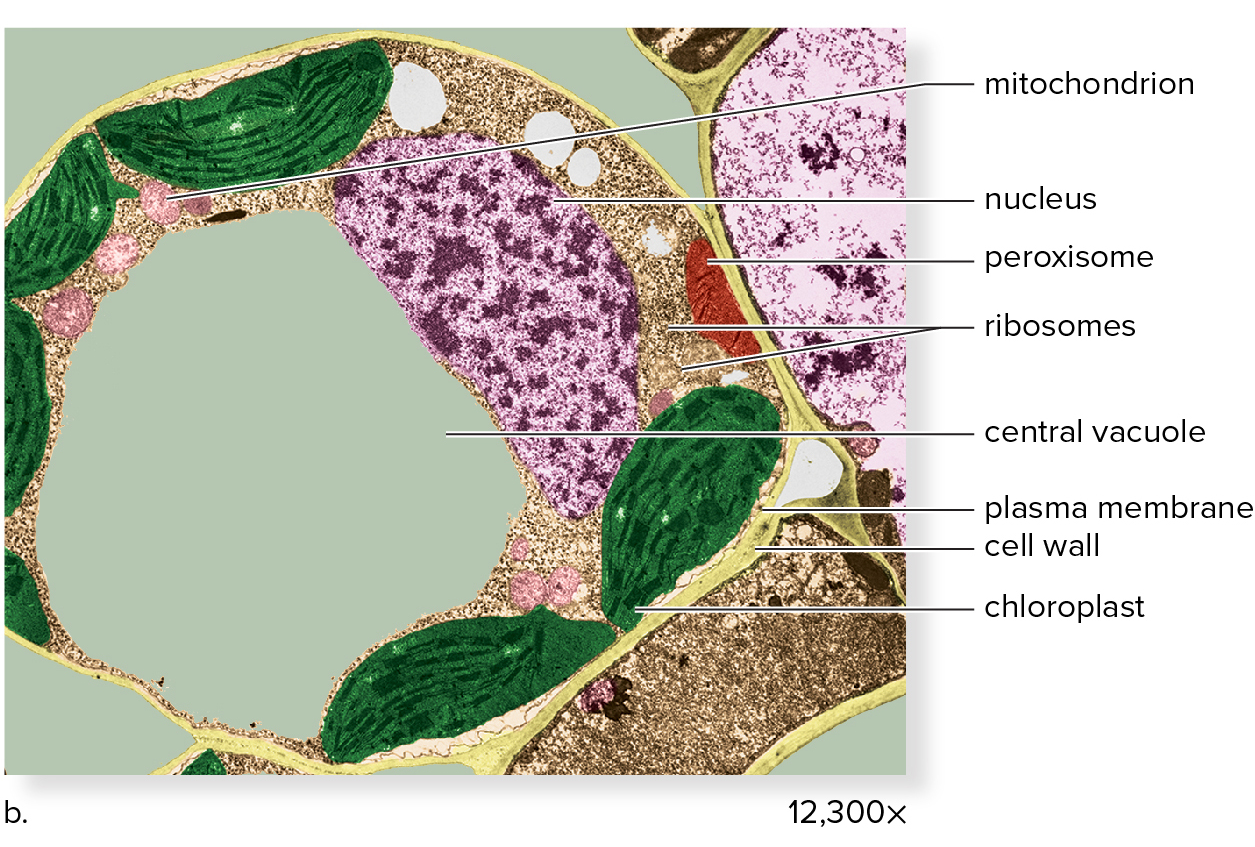
\includegraphics[width=0.5\linewidth]{Vacuole}
	\caption[Vacuole]{Vacuole}
	\label{fig:vacuole}
\end{figure}

\subsubsection{Energie-organellen}
\paragraph{Mitochondriën}
Mitochondriën vinden we zowel in planten als dieren, ze zijn erg klein waardoor ze enkel te zien zijn met een elektronenmicroscoop. Ze hebben een dubbelmembraan waarbij de binnenste membraan een groter oppervlak heeft dan de buitenste. Dit betekend dat er plooien moeten komen in het binnenste membraan, deze plooien noemen we cristae. Binnenin zit de matrix, dit bevat enzymen die koolhydraatafbraak ondersteunen, om dan ATP te synthetiseren. Verdere functies van Mitochondriën worden verduidelijkt in sectie \textcolor{red}{TEMP-REF TO ENERGY CELLS}.
\begin{figure}[h!]
	\centering
	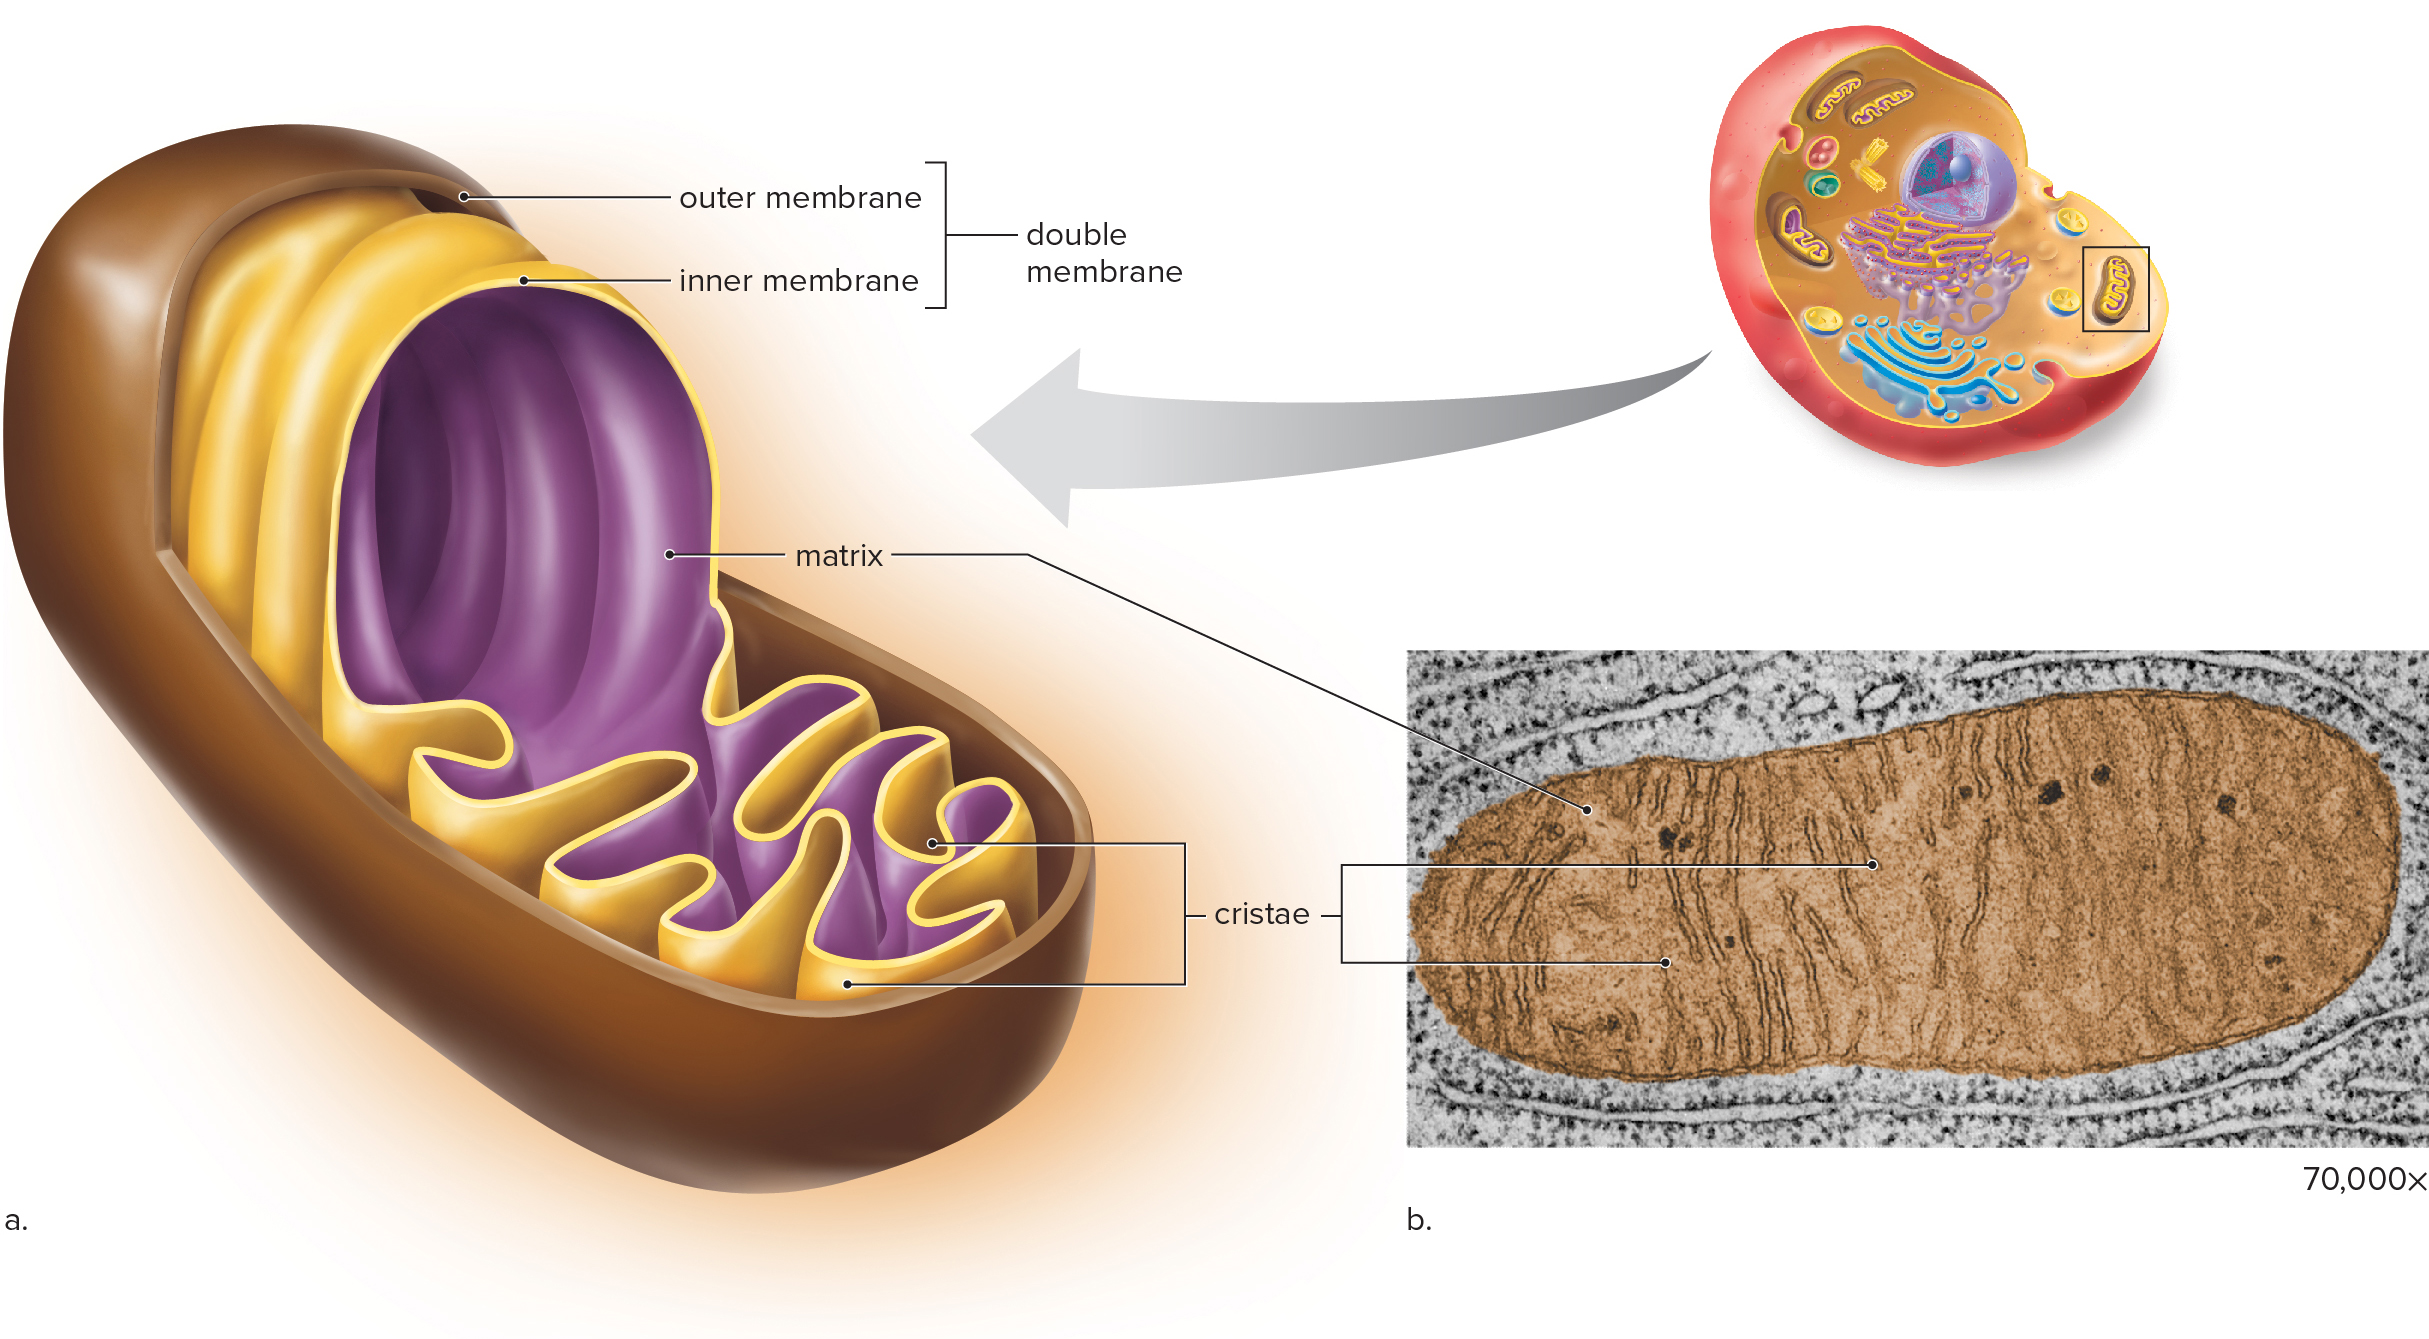
\includegraphics[width=0.7\linewidth]{PowerhouseOfTheCell}
	\caption[Mitochondria]{Mitochondriën: The Powerhouse of The Cel!}
	\label{fig:powerhouseofthecell}
\end{figure}

\paragraph{Chloroplasten}
\subsubsection{Cytoskelet}
\subsubsection{Centriolen}
\subsubsection{Cilia en flagellen}
\subsection{Extracellulaire structuren}
\subsubsection{Celwand}
\subsubsection{Extracellulaire matrix}
\subsubsection{Juncties tussen cellen}
\subsection{Wat met virussen?}


\end{document}
